%%%%%%%%%%%%%%%%%%%%%%%%%%%%%%%%%%%%%%%%%
%  My documentation report
%  Objetive: Explain what I did and how, so someone can continue with the investigation
%
% Important note:
% Chapter heading images should have a 2:1 width:height ratio,
% e.g. 920px width and 460px height.
%
%%%%%%%%%%%%%%%%%%%%%%%%%%%%%%%%%%%%%%%%%

%----------------------------------------------------------------------------------------
%	PACKAGES AND OTHER DOCUMENT CONFIGURATIONS
%----------------------------------------------------------------------------------------

\documentclass[11pt,fleqn]{book} % Default font size and left-justified equations

\usepackage[top=3cm,bottom=3cm,left=3.2cm,right=3.2cm,headsep=10pt,a4paper]{geometry} % Page margins

\usepackage{xcolor} % Required for specifying colors by name
\definecolor{ocre}{RGB}{52,177,201} % Define the orange color used for highlighting throughout the book

% Font Settings
\usepackage{avant} % Use the Avantgarde font for headings
%\usepackage{times} % Use the Times font for headings
\usepackage{mathptmx} % Use the Adobe Times Roman as the default text font together with math symbols from the Sym­bol, Chancery and Com­puter Modern fonts

\usepackage{microtype} % Slightly tweak font spacing for aesthetics
\usepackage[utf8]{inputenc} % Required for including letters with accents
\usepackage[T1]{fontenc} % Use 8-bit encoding that has 256 glyphs

% Bibliography
%\usepackage[style=alphabetic,sorting=nyt,sortcites=true,autopunct=true,babel=hyphen,hyperref=true,abbreviate=false,backref=true,backend=biber]{biblatex}
%\addbibresource{bibliography.bib} % BibTeX bibliography file
%\defbibheading{bibempty}{}

%----------------------------------------------------------------------------------------
%	VARIOUS REQUIRED PACKAGES
%----------------------------------------------------------------------------------------

\usepackage{titlesec} % Allows customization of titles

\usepackage{graphicx} % Required for including pictures
\graphicspath{{Pictures/}} % Specifies the directory where pictures are stored

\usepackage{lipsum} % Inserts dummy text

\usepackage{tikz} % Required for drawing custom shapes

%\usepackage[english]{babel} % English language/hyphenation
\usepackage[brazil]{babel}

\usepackage{enumitem} % Customize lists
\setlist{nolistsep} % Reduce spacing between bullet points and numbered lists

\usepackage{booktabs} % Required for nicer horizontal rules in tables

\usepackage{eso-pic} % Required for specifying an image background in the title page

%----------------------------------------------------------------------------------------
%	MAIN TABLE OF CONTENTS
%----------------------------------------------------------------------------------------

\usepackage{titletoc} % Required for manipulating the table of contents

\contentsmargin{0cm} % Removes the default margin
% Chapter text styling
\titlecontents{chapter}[1.25cm] % Indentation
{\addvspace{15pt}\large\sffamily\bfseries} % Spacing and font options for chapters
{\color{ocre!60}\contentslabel[\Large\thecontentslabel]{1.25cm}\color{ocre}} % Chapter number
{}  
{\color{ocre!60}\normalsize\sffamily\bfseries\;\titlerule*[.5pc]{.}\;\thecontentspage} % Page number
% Section text styling
\titlecontents{section}[1.25cm] % Indentation
{\addvspace{5pt}\sffamily\bfseries} % Spacing and font options for sections
{\contentslabel[\thecontentslabel]{1.25cm}} % Section number
{}
{\sffamily\hfill\color{black}\thecontentspage} % Page number
[]
% Subsection text styling
\titlecontents{subsection}[1.25cm] % Indentation
{\addvspace{1pt}\sffamily\small} % Spacing and font options for subsections
{\contentslabel[\thecontentslabel]{1.25cm}} % Subsection number
{}
{\sffamily\;\titlerule*[.5pc]{.}\;\thecontentspage} % Page number
[] 

%----------------------------------------------------------------------------------------
%	MINI TABLE OF CONTENTS IN CHAPTER HEADS
%----------------------------------------------------------------------------------------

% Section text styling
\titlecontents{lsection}[0em] % Indendating
{\footnotesize\sffamily} % Font settings
{}
{}
{}

% Subsection text styling
\titlecontents{lsubsection}[.5em] % Indentation
{\normalfont\footnotesize\sffamily} % Font settings
{}
{}
{}
 
%----------------------------------------------------------------------------------------
%	PAGE HEADERS
%----------------------------------------------------------------------------------------

\usepackage{fancyhdr} % Required for header and footer configuration

\pagestyle{fancy}
\renewcommand{\chaptermark}[1]{\markboth{\sffamily\normalsize\bfseries\chaptername\ \thechapter.\ #1}{}} % Chapter text font settings
\renewcommand{\sectionmark}[1]{\markright{\sffamily\normalsize\thesection\hspace{5pt}#1}{}} % Section text font settings
\fancyhf{} \fancyhead[LE,RO]{\sffamily\normalsize\thepage} % Font setting for the page number in the header
\fancyhead[LO]{\rightmark} % Print the nearest section name on the left side of odd pages
\fancyhead[RE]{\leftmark} % Print the current chapter name on the right side of even pages
\renewcommand{\headrulewidth}{0.5pt} % Width of the rule under the header
\addtolength{\headheight}{2.5pt} % Increase the spacing around the header slightly
\renewcommand{\footrulewidth}{0pt} % Removes the rule in the footer
\fancypagestyle{plain}{\fancyhead{}\renewcommand{\headrulewidth}{0pt}} % Style for when a plain pagestyle is specified

% Removes the header from odd empty pages at the end of chapters
\makeatletter
\renewcommand{\cleardoublepage}{
\clearpage\ifodd\c@page\else
\hbox{}
\vspace*{\fill}
\thispagestyle{empty}
\newpage
\fi}

%----------------------------------------------------------------------------------------
%	THEOREM STYLES
%----------------------------------------------------------------------------------------

\usepackage{amsmath,amsfonts,amssymb,amsthm} % For math equations, theorems, symbols, etc

\newcommand{\intoo}[2]{\mathopen{]}#1\,;#2\mathclose{[}}
\newcommand{\ud}{\mathop{\mathrm{{}d}}\mathopen{}}
\newcommand{\intff}[2]{\mathopen{[}#1\,;#2\mathclose{]}}
\newtheorem{notation}{Notation}[chapter]

%%%%%%%%%%%%%%%%%%%%%%%%%%%%%%%%%%%%%%%%%%%%%%%%%%%%%%%%%%%%%%%%%%%%%%%%%%%
%%%%%%%%%%%%%%%%%%%% dedicated to boxed/framed environements %%%%%%%%%%%%%%
%%%%%%%%%%%%%%%%%%%%%%%%%%%%%%%%%%%%%%%%%%%%%%%%%%%%%%%%%%%%%%%%%%%%%%%%%%%
\newtheoremstyle{ocrenumbox}% % Theorem style name
{0pt}% Space above
{0pt}% Space below
{\normalfont}% % Body font
{}% Indent amount
{\small\bf\sffamily\color{ocre}}% % Theorem head font
{\;}% Punctuation after theorem head
{0.25em}% Space after theorem head
{\small\sffamily\color{ocre}\thmname{#1}\nobreakspace\thmnumber{\@ifnotempty{#1}{}\@upn{#2}}% Theorem text (e.g. Theorem 2.1)
\thmnote{\nobreakspace\the\thm@notefont\sffamily\bfseries\color{black}---\nobreakspace#3.}} % Optional theorem note
\renewcommand{\qedsymbol}{$\blacksquare$}% Optional qed square

\newtheoremstyle{blacknumex}% Theorem style name
{5pt}% Space above
{5pt}% Space below
{\normalfont}% Body font
{} % Indent amount
{\small\bf\sffamily}% Theorem head font
{\;}% Punctuation after theorem head
{0.25em}% Space after theorem head
{\small\sffamily{\tiny\ensuremath{\blacksquare}}\nobreakspace\thmname{#1}\nobreakspace\thmnumber{\@ifnotempty{#1}{}\@upn{#2}}% Theorem text (e.g. Theorem 2.1)
\thmnote{\nobreakspace\the\thm@notefont\sffamily\bfseries---\nobreakspace#3.}}% Optional theorem note

\newtheoremstyle{blacknumbox} % Theorem style name
{0pt}% Space above
{0pt}% Space below
{\normalfont}% Body font
{}% Indent amount
{\small\bf\sffamily}% Theorem head font
{\;}% Punctuation after theorem head
{0.25em}% Space after theorem head
{\small\sffamily\thmname{#1}\nobreakspace\thmnumber{\@ifnotempty{#1}{}\@upn{#2}}% Theorem text (e.g. Theorem 2.1)
\thmnote{\nobreakspace\the\thm@notefont\sffamily\bfseries---\nobreakspace#3.}}% Optional theorem note

%%%%%%%%%%%%%%%%%%%%%%%%%%%%%%%%%%%%%%%%%%%%%%%%%%%%%%%%%%%%%%%%%%%%%%%%%%%
%%%%%%%%%%%%% dedicated to non-boxed/non-framed environements %%%%%%%%%%%%%
%%%%%%%%%%%%%%%%%%%%%%%%%%%%%%%%%%%%%%%%%%%%%%%%%%%%%%%%%%%%%%%%%%%%%%%%%%%
\newtheoremstyle{ocrenum}% % Theorem style name
{5pt}% Space above
{5pt}% Space below
{\normalfont}% % Body font
{}% Indent amount
{\small\bf\sffamily\color{ocre}}% % Theorem head font
{\;}% Punctuation after theorem head
{0.25em}% Space after theorem head
{\small\sffamily\color{ocre}\thmname{#1}\nobreakspace\thmnumber{\@ifnotempty{#1}{}\@upn{#2}}% Theorem text (e.g. Theorem 2.1)
\thmnote{\nobreakspace\the\thm@notefont\sffamily\bfseries\color{black}---\nobreakspace#3.}} % Optional theorem note
\renewcommand{\qedsymbol}{$\blacksquare$}% Optional qed square
\makeatother

% Defines the theorem text style for each type of theorem to one of the three styles above
\newcounter{dummy} 
\numberwithin{dummy}{section}
\theoremstyle{ocrenumbox}
\newtheorem{theoremeT}[dummy]{Theorem}
\newtheorem{problem}{Problem}[chapter]
\newtheorem{exerciseT}{Exercise}[chapter]
\theoremstyle{blacknumex}
\newtheorem{exampleT}{Example}[chapter]
\theoremstyle{blacknumbox}
\newtheorem{vocabulary}{Vocabulary}[chapter]
\newtheorem{definitionT}{Definition}[section]
\newtheorem{corollaryT}[dummy]{Corollary}
\theoremstyle{ocrenum}
\newtheorem{proposition}[dummy]{Proposition}

%----------------------------------------------------------------------------------------
%	DEFINITION OF COLORED BOXES
%----------------------------------------------------------------------------------------

\RequirePackage[framemethod=default]{mdframed} % Required for creating the theorem, definition, exercise and corollary boxes

% Theorem box
\newmdenv[skipabove=7pt,
skipbelow=7pt,
backgroundcolor=black!5,
linecolor=ocre,
innerleftmargin=5pt,
innerrightmargin=5pt,
innertopmargin=5pt,
leftmargin=0cm,
rightmargin=0cm,
innerbottommargin=5pt]{tBox}

% Exercise box	  
\newmdenv[skipabove=7pt,
skipbelow=7pt,
rightline=false,
leftline=true,
topline=false,
bottomline=false,
backgroundcolor=ocre!10,
linecolor=ocre,
innerleftmargin=5pt,
innerrightmargin=5pt,
innertopmargin=5pt,
innerbottommargin=5pt,
leftmargin=0cm,
rightmargin=0cm,
linewidth=4pt]{eBox}	

% Definition box
\newmdenv[skipabove=7pt,
skipbelow=7pt,
rightline=false,
leftline=true,
topline=false,
bottomline=false,
linecolor=ocre,
innerleftmargin=5pt,
innerrightmargin=5pt,
innertopmargin=0pt,
leftmargin=0cm,
rightmargin=0cm,
linewidth=4pt,
innerbottommargin=0pt]{dBox}	

% Corollary box
\newmdenv[skipabove=7pt,
skipbelow=7pt,
rightline=false,
leftline=true,
topline=false,
bottomline=false,
linecolor=gray,
backgroundcolor=black!5,
innerleftmargin=5pt,
innerrightmargin=5pt,
innertopmargin=5pt,
leftmargin=0cm,
rightmargin=0cm,
linewidth=4pt,
innerbottommargin=5pt]{cBox}

% Creates an environment for each type of theorem and assigns it a theorem text style from the "Theorem Styles" section above and a colored box from above
\newenvironment{theorem}{\begin{tBox}\begin{theoremeT}}{\end{theoremeT}\end{tBox}}
\newenvironment{exercise}{\begin{eBox}\begin{exerciseT}}{\hfill{\color{ocre}\tiny\ensuremath{\blacksquare}}\end{exerciseT}\end{eBox}}				  
\newenvironment{definition}{\begin{dBox}\begin{definitionT}}{\end{definitionT}\end{dBox}}	
\newenvironment{example}{\begin{exampleT}}{\hfill{\tiny\ensuremath{\blacksquare}}\end{exampleT}}		
\newenvironment{corollary}{\begin{cBox}\begin{corollaryT}}{\end{corollaryT}\end{cBox}}	

%----------------------------------------------------------------------------------------
%	REMARK ENVIRONMENT
%----------------------------------------------------------------------------------------

\newenvironment{remark}{\par\vspace{10pt}\small % Vertical white space above the remark and smaller font size
\begin{list}{}{
\leftmargin=35pt % Indentation on the left
\rightmargin=25pt}\item\ignorespaces % Indentation on the right
\makebox[-2.5pt]{\begin{tikzpicture}[overlay]
\node[draw=ocre!60,line width=1pt,circle,fill=ocre!25,font=\sffamily\bfseries,inner sep=2pt,outer sep=0pt] at (-15pt,0pt){\textcolor{ocre}{R}};\end{tikzpicture}} % Orange R in a circle
\advance\baselineskip -1pt}{\end{list}\vskip5pt} % Tighter line spacing and white space after remark

%----------------------------------------------------------------------------------------
%	SECTION NUMBERING IN THE MARGIN
%----------------------------------------------------------------------------------------

\makeatletter
\renewcommand{\@seccntformat}[1]{\llap{\textcolor{ocre}{\csname the#1\endcsname}\hspace{1em}}}                    
\renewcommand{\section}{\@startsection{section}{1}{\z@}
{-4ex \@plus -1ex \@minus -.4ex}
{1ex \@plus.2ex }
{\normalfont\large\sffamily\bfseries}}
\renewcommand{\subsection}{\@startsection {subsection}{2}{\z@}
{-3ex \@plus -0.1ex \@minus -.4ex}
{0.5ex \@plus.2ex }
{\normalfont\sffamily\bfseries}}
\renewcommand{\subsubsection}{\@startsection {subsubsection}{3}{\z@}
{-2ex \@plus -0.1ex \@minus -.2ex}
{.2ex \@plus.2ex }
{\normalfont\small\sffamily\bfseries}}                        
\renewcommand\paragraph{\@startsection{paragraph}{4}{\z@}
{-2ex \@plus-.2ex \@minus .2ex}
{.1ex}
{\normalfont\small\sffamily\bfseries}}

%----------------------------------------------------------------------------------------
%	HYPERLINKS IN THE DOCUMENTS
%----------------------------------------------------------------------------------------

% For an unclear reason, the package should be loaded now and not later
\usepackage{hyperref}
\hypersetup{hidelinks,backref=true,pagebackref=true,hyperindex=true,colorlinks=false,breaklinks=true,urlcolor= ocre,bookmarks=true,bookmarksopen=false,pdftitle={Title},pdfauthor={Author}}

%----------------------------------------------------------------------------------------
%	CHAPTER HEADINGS
%----------------------------------------------------------------------------------------

% The set-up below should be (sadly) manually adapted to the overall margin page septup controlled by the geometry package loaded in the main.tex document. It is possible to implement below the dimensions used in the goemetry package (top,bottom,left,right)... TO BE DONE

\newcommand{\thechapterimage}{}
\newcommand{\chapterimage}[1]{\renewcommand{\thechapterimage}{#1}}

% Numbered chapters with mini tableofcontents
\def\thechapter{\arabic{chapter}}
\def\@makechapterhead#1{
\thispagestyle{empty}
{\centering \normalfont\sffamily
\ifnum \c@secnumdepth >\m@ne
\if@mainmatter
\startcontents
\begin{tikzpicture}[remember picture,overlay]
\node at (current page.north west)
{\begin{tikzpicture}[remember picture,overlay]
\node[anchor=north west,inner sep=0pt] at (0,0) {\includegraphics[width=\paperwidth]{\thechapterimage}};
%%%%%%%%%%%%%%%%%%%%%%%%%%%%%%%%%%%%%%%%%%%%%%%%%%%%%%%%%%%%%%%%%%%%%%%%%%%%%%%%%%%%%
% Commenting the 3 lines below removes the small contents box in the chapter heading
%\fill[color=ocre!10!white,opacity=.6] (1cm,0) rectangle (8cm,-7cm);
%\node[anchor=north west] at (1.1cm,.35cm) {\parbox[t][8cm][t]{6.5cm}{\huge\bfseries\flushleft \printcontents{l}{1}{\setcounter{tocdepth}{2}}}};
\draw[anchor=west] (5cm,-9cm) node [rounded corners=20pt,fill=ocre!10!white,text opacity=1,draw=ocre,draw opacity=1,line width=1.5pt,fill opacity=.6,inner sep=12pt]{\huge\sffamily\bfseries\textcolor{black}{\thechapter. #1\strut\makebox[22cm]{}}};
%%%%%%%%%%%%%%%%%%%%%%%%%%%%%%%%%%%%%%%%%%%%%%%%%%%%%%%%%%%%%%%%%%%%%%%%%%%%%%%%%%%%%
\end{tikzpicture}};
\end{tikzpicture}}
\par\vspace*{230\p@}
\fi
\fi}

% Unnumbered chapters without mini tableofcontents (could be added though) 
\def\@makeschapterhead#1{
\thispagestyle{empty}
{\centering \normalfont\sffamily
\ifnum \c@secnumdepth >\m@ne
\if@mainmatter
\begin{tikzpicture}[remember picture,overlay]
\node at (current page.north west)
{\begin{tikzpicture}[remember picture,overlay]
\node[anchor=north west,inner sep=0pt] at (0,0) {\includegraphics[width=\paperwidth]{\thechapterimage}};
\draw[anchor=west] (5cm,-9cm) node [rounded corners=20pt,fill=ocre!10!white,fill opacity=.6,inner sep=12pt,text opacity=1,draw=ocre,draw opacity=1,line width=1.5pt]{\huge\sffamily\bfseries\textcolor{black}{#1\strut\makebox[22cm]{}}};
\end{tikzpicture}};
\end{tikzpicture}}
\par\vspace*{230\p@}
\fi
\fi
}
\makeatother
 % Insert the commands.tex file which contains the majority of the structure behind the template

%\usepackage[portuges]{babel}
\usepackage{float} %NEW
\usepackage{breakurl}

\usepackage{parskip}

\begin{document}


\thispagestyle{plain} % empty
\mbox{}
\newpage
%----------------------------------------------------------------------------------------
%	TITLE PAGE
%----------------------------------------------------------------------------------------

\begingroup
\thispagestyle{empty}
\AddToShipoutPicture*{\put(0,0){
\includegraphics[scale=0.65]{Capa1.png}}} % Image background
%\AddToShipoutPicture*{\put(0,0){\includegraphics[scale=1.25]{esahubble}}} % Image background
\centering
\vspace*{5cm}
\par\normalfont\fontsize{35}{35}\sffamily\selectfont

\textbf{Guia do Thunkable}
%
\includegraphics[width=0.5\textwidth]{logothunk.png}\\
{\LARGE Crie seus aplicativos para smartphone!}\par % Book title
\vspace*{1cm}
{\Large Clube de Computação -- UFSM\\~ \\
facebook.com/CombClubUFSM\\
compclub@inf.ufsm.br\\}%\par % Author name
\endgroup

%----------------------------------------------------------------------------------------
%	COPYRIGHT PAGE
%----------------------------------------------------------------------------------------
\setlength\parindent{0pt}
\setlength{\parskip}{11pt}

\newpage
~\vfill
\thispagestyle{empty}

%\noindent Copyright \copyright\ 2014 Andrea Hidalgo\\ % Copyright notice

\noindent \textsc{Universidade Federal de Santa Maria -- UFSM\\
 Centro de Tecnologia -- CT\\ Departamento de Linguagens e Sistemas de Computação -- DLSC}\\

\noindent \textsc{Apresentação}\\ % URL

\noindent Este guia foi desenvolvido pela equipe do Clube de Computação da UFSM, programa de extensão que visa disseminar fundamentos da programação de computadores e do pensamento computacional a estudantes do ensino fundamental e médio. Através deste guia, queremos apresentar o Thunkable, uma ferramenta para criação de aplicativos de maneira simplificada, usando encaixe de blocos semelhantes a quebra-cabeças. O Thunkable baseia-se em uma ferramenta precursora, chamada MIT App Inventor, que foi utilizada pelo Clube de Computação entre 2015 e 2016 e apresentada em outro guia que elaboramos anteriormente a este. Neste novo guia, mantivemos alguns textos e exemplos do guia anterior, porém utilizamos uma ferramenta mais moderna que traz novas opções. Ambos os guias foram elaborados com apoio do Fundo de Incentivo à Extensão (FIEX) da Universidade Federal de Santa Maria.
\\ % License information

\vspace{1cm}
\noindent Participaram da criação deste guia:

%\vspace{1cm}


\begin{itemize}
\item Profª Andrea Schwertner Charão -- Coordenadora (DLSC/UFSM)
\end{itemize}

\noindent Tutores -- Alunos de Graduação da UFSM:

\begin{itemize}

\item Jéferson Marques da Silva -- Sistemas de Informação
\item Lana Bertoldo Rossato -- Ciência da Computação
\item Miguel Miron Silva -- Ciência da Computação
\item Paulo Stoll -- Ciência da Computação
\item Viviane Dilkin Endler -- Bolsista FIEX / Ciência da Computação
\end{itemize}

\vspace{1cm}

\noindent Agradecemos aos tutores que colaboraram na elaboração do Guia do MIT App Inventor em 2016 (Ana Luísa Veroneze Solórzano, Pedro Prestes Matiuzzi) e em 2015 (Ana Luísa Veroneze Solórzano, Cassiano Andrei Dias da Silveira Schneider, Daniel Matheus Doebber, Filipe Simões Mendonça, Iago da Cunha Corrêa, Lucas Ferreira da Silva, Lucas de Oliveira Dias, Luísa Perin Lucca, Rafael Gauna Trindade e Vinícius Mateus Dreifke).


\vspace{1cm}

\noindent \textit{Primeira edição, Outubro de 2019} % Printing/edition date

\vspace{1cm}

\cleardoublepage

%\newpage
%\thispagestyle{plain} % empty
%\mbox{}

%----------------------------------------------------------------------------------------
%	TABLE OF CONTENTS
%----------------------------------------------------------------------------------------

\chapterimage{Capa8.png} % Table of contents heading image

\pagestyle{empty} % No headers

\tableofcontents % Print the table of contents itself

\cleardoublepage % Forces the first chapter to start on an odd page so it's on the right

\pagestyle{fancy} % Print headers again

%----------------------------------------------------------------------------------------
%	CHAPTER 1
%----------------------------------------------------------------------------------------

\chapterimage{Capa1.png} % Chapter heading image

\chapter{Primeiro contato com o Thunkable?}\label{ch:thunkable}

\section{Primeiros passos}\index{PPassos}
Aqui você vai aprender passo a passo como começar a utilizar essa ferramenta! Explicaremos como iniciar a criação de um novo projeto, ou seja, um novo aplicativo.

%\remark{teste}
Antes de mais nada: \textbf{O Thunkable requer que você tenha uma conta de e-mail, por isso não esqueça de criá-la antes!}

Para começar, acesse o site do Thunkable (\url{https://x.thunkable.com}) e você verá a página principal de login (Figura \ref{fig:guia1}).

\begin{figure}[h]
    \centering
    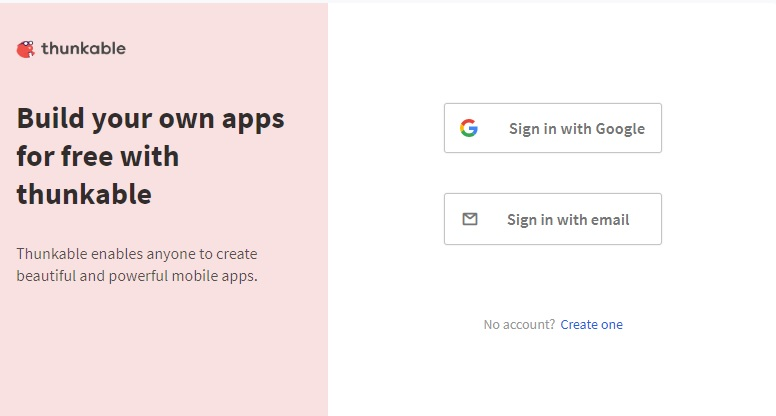
\includegraphics[width=0.9\textwidth]{GuiaThunkSignIn.jpg}
    \caption{Tela de login do Thunkable}\label{fig:guia1}
\end{figure}



Se você tem conta no Gmail, clique em ``Sign in with Google'', senão escolha ``Sign in with email'' e entre com os dados da sua conta de e-mail. Se você já está logado, confirme que esta é de fato a conta que você deseja usar.

 
% Para usar o App Inventor você deve concordar com os Termos de Serviço da ferramenta clicando em \textit{I accepted the terms of service!}. Você será convidado para responder uma pesquisa, podendo decidir respondê-la em outro momento (\textit{Take Survey Later}). Após, uma mensagem de boas vindas aparecerá, nela você poderá saber um pouco mais sobre as formas de executar o seu aplicativo:

No seu primeiro acesso, aparecerá uma tela de boas-vindas com uma sequência de informações sobre o Thunkable (Figura \ref{fig:welcome}).

\begin{figure}[H]
    \centering
    %\includegraphics[width=0.77\textwidth]{GuiaApp3.jpg}
    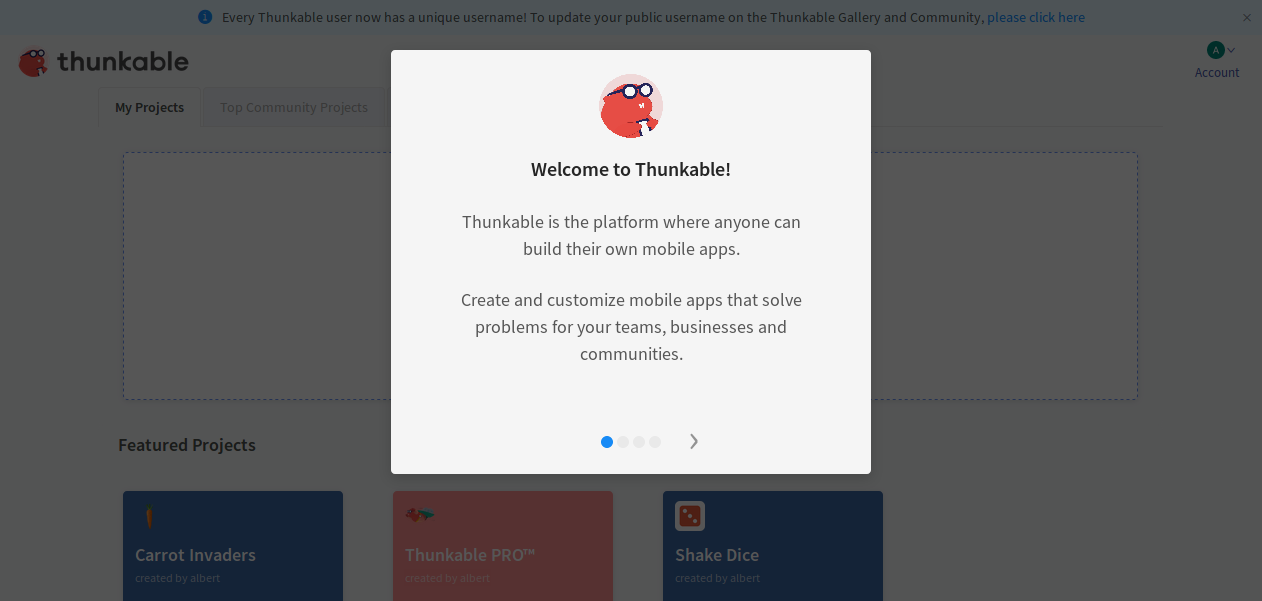
\includegraphics[width=0.77\textwidth]{GuiaThunk1Welcome.png}
    \caption{Tela de boas-vindas do Thunkable}\label{fig:welcome}
\end{figure}

Ao final da sequência de boas-vindas, você poderá iniciar a criação do seu aplicativo clicando em ``Start Building'' (iniciar construção), conforme mostra a Figura \ref{fig:start}.

%clique em \textit{Create New App!} (``Criar um novo aplicativo!'').

\begin{figure}[H]
    \centering
    %\includegraphics[width=0.77\textwidth]{GuiaApp3.jpg}
    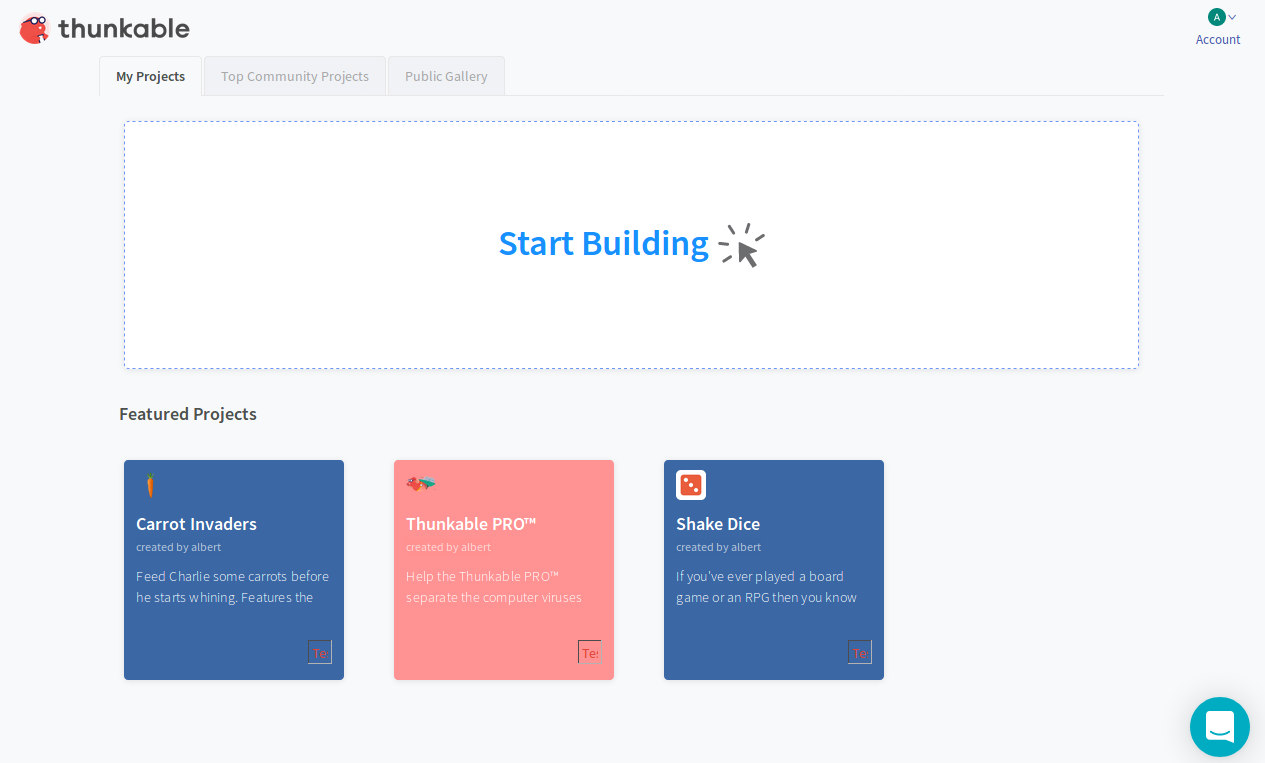
\includegraphics[width=0.77\textwidth]{GuiaThunk1Start.png}
    \caption{Tela inicial do Thunkable}\label{fig:start}
\end{figure}

Cada aplicativo será um novo projeto (Project), ao qual você deverá dar um nome (Figura \ref{fig:newproject}).

\begin{figure}[H]
    \centering
    %\includegraphics[width=0.77\textwidth]{GuiaApp3.jpg}
    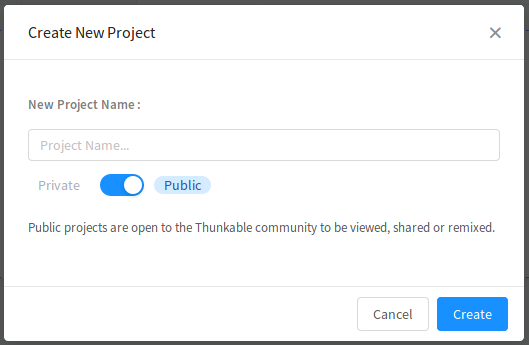
\includegraphics[width=0.5\textwidth]{GuiaThunk1NewProject.png}
    \caption{Tela de criação de projeto no Thunkable}\label{fig:newproject}
\end{figure}

Quando você já tiver começado a criar um aplicativo, as telas de primeiro acesso não aparecerão mais. Você irá diretamente para uma tela que mostrará um painel com seus projetos (My Projects) e também com alguns projetos em destaque (Featured Projects), que você pode usar como exemplo. Nesta tela, também encontra-se a opção de criar um novo projeto (Create New App).

\begin{figure}[H]
    \centering
    %\includegraphics[width=0.77\textwidth]{GuiaApp3.jpg}
    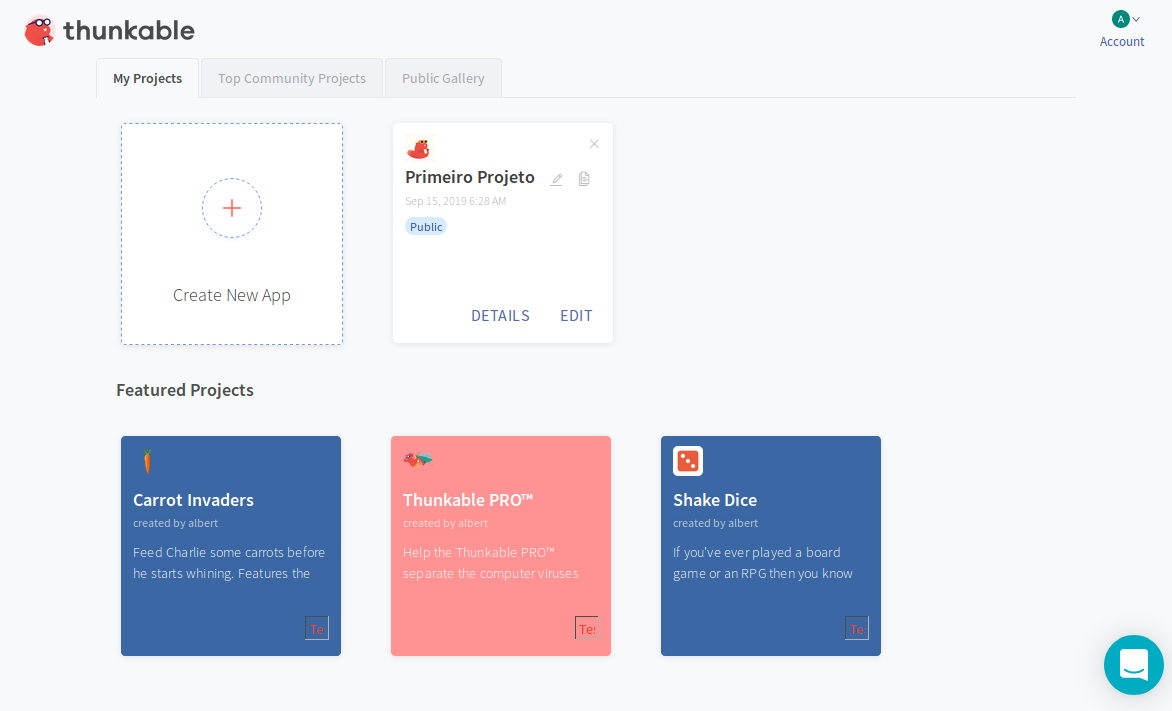
\includegraphics[width=0.77\textwidth]{GuiaThunk1MyProjects.png}
    \caption{Tela com painel de projetos no Thunkable}\label{fig:myprojects}
\end{figure}

% 1 - Utilizando um dispositivo móvel com Android

% 2 - Utilizando o emulador de Android

% \textbf{No capítulo~\ref{ch:teste} você aprenderá como executar o seu aplicativo em cada caso.} 

%------------------------------------------------

\section{Conhecendo o ambiente de trabalho}\index{Ambiente}

%Que tal começar mudando o idioma para português?
Quando você criar um novo projeto de aplicativo, finalmente você vai ver uma tela com as várias opções do Thunkable, divididas em algumas áreas que você precisará distinguir (Figura \ref{fig:areas}). Estas áreas podem ser redimensionadas clicando-se nas linhas divisórias. Logo no início da criação de um projeto, aparece uma área de tutoriais bem à esquerda (Hour of Code Tutorials). Você pode esconder esta área enquanto estiver seguindo este nosso guia em português.

\begin{figure}[H]
    \centering
    %\includegraphics[width=0.77\textwidth]{GuiaApp4.jpg}
    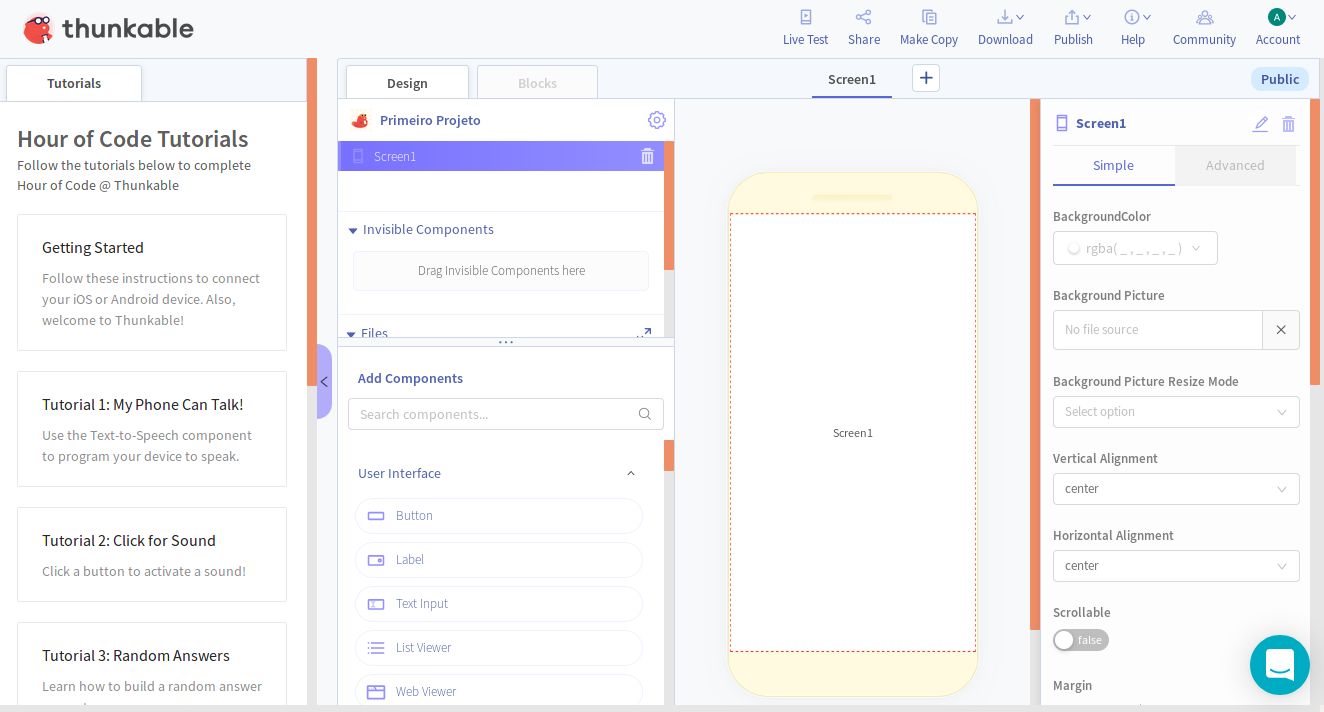
\includegraphics[width=0.77\textwidth]{GuiaThunk1Areas.png}
    \caption{Tela do Thunkable dividida em áreas}\label{fig:areas}
\end{figure}

Enquanto você estiver criando um aplicativo, você precisará alternar entre 2 perspectivas: Design e Blocks. Estas perspectivas são selecionáveis em abas e correspondem a diferentes telas de criação do aplicativo. A tela \textbf{Design} é a aba selecionada por padrão, logo que você inicia o projeto. Esta tela tem várias opções para organizar o visual do seu aplicativo. A tela \textbf{Blocks}, por sua vez, tem opções de programação do aplicativo, usando uma linguagem visual de encaixe de blocos. Nas seções seguintes, você vai conhecer melhor cada uma dessas telas.


\subsection{Tela Design} 
Na tela Design (Figura \ref{fig:teladesign}), você vai criar as telas do seu aplicativo. Logo no início da criação do aplicativo, o Thunkable já cria uma tela padrão (Screen1), que está vazia. Você deverá preencher esta tela do aplicativo conforme desejar, usando vários componentes que podem ser adicionados e configurados. A seguir explicaremos um pouco mais sobre cada área da tela Design.

\begin{figure}[H]
    \centering
    %\includegraphics[width=0.77\textwidth]{GuiaApp5.jpg}
    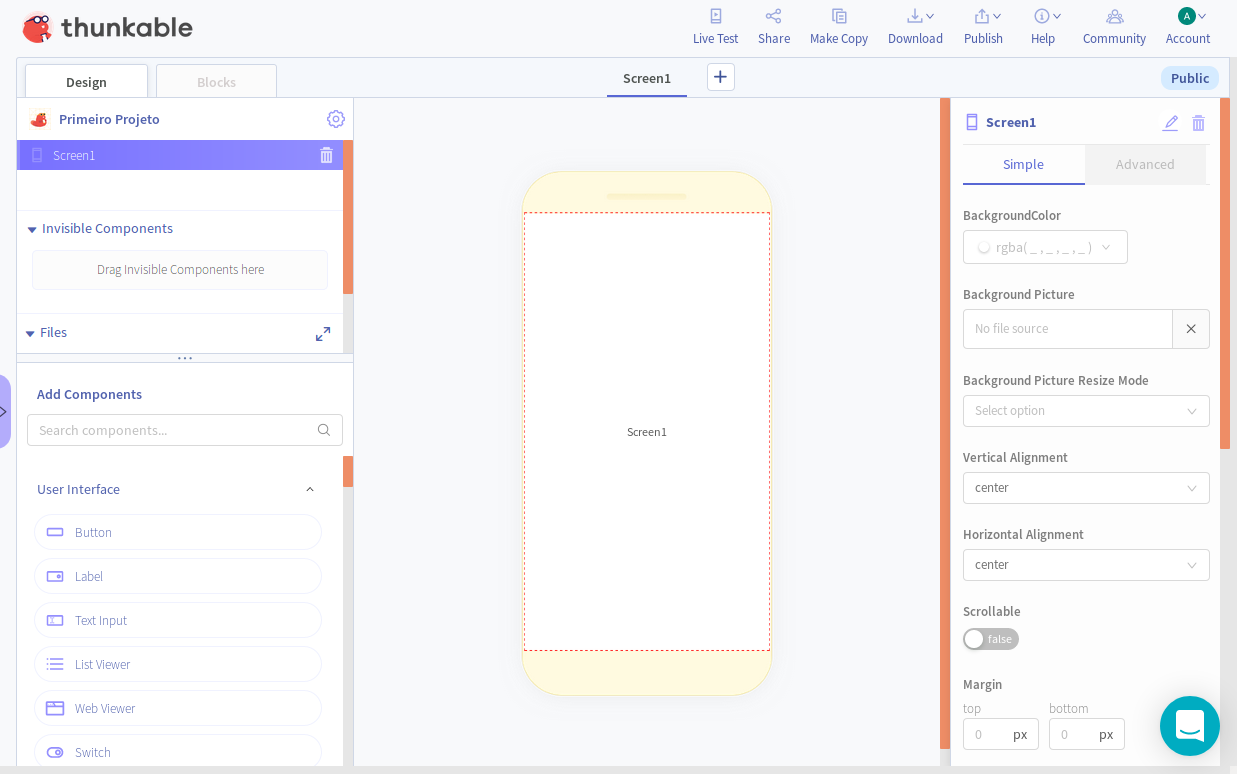
\includegraphics[width=0.8\textwidth]{GuiaThunk1Design.png}
    \caption{Tela Design}\label{fig:teladesign}
\end{figure}

\begin{itemize}
\item Estrutura do aplicativo: na área superior à esquerda, existe uma área ajustável com o nome do seu projeto e com sua estrutura, isto é, a hierarquia de componentes que fazem parte do aplicativo (inicialmente, somente uma tela, Screen1). Conforme você for adicionando componentes, esta área vai aumentar e você precisará usar a barra de rolagem. Você também poderá esconder/revelar as seções desta área, marcadas com triângulos (Screen1, Invisible Components, Files, etc.), alternando entre visões condensada ou ampliada de cada seção.


\item Menu de componentes (Add Components): esta área é situada logo abaixo da área anterior. Ela oferece uma grande variedade de componentes visuais (ou não), que podem ser adicionados a seu aplicativo. Você poderá usar a barra de rolagem para navegar pelas opções, ou usar a caixa de busca quando souber o nome do componente. Para adicionar um componente, você deve selecioná-lo e arrastá-lo para a tela em edição ou para a área com a estrutura do seu aplicativo.

\item Tela em edição: na área central da tela Design, é mostrada a tela em edição, oferecendo uma ideia de como o aplicativo irá aparecer no smartphone. Você pode reorganizar os componentes na tela, usando o mouse para arrastar e soltar componentes. Quando selecionar um componente, este será destacado na área de estrutura do aplicativo e também na área de propriedades, descrita a seguir.


\item Propriedades: esta área situa-se à direita da tela Design e mostra as propriedades do componente selecionado. Cada componente tem várias propriedades que configuram seu aspecto. Por exemplo, um botão (Button) tem propriedades que ajustam seu texto, sua cor de frente/fundo, suas dimensões (Height e Width, isto é, altura e largura), sua borda, etc. Muitos nomes de propriedades estão presentes em diferentes componentes. Para evitar confusão, verifique sempre o componente que está selecionado.



\end{itemize}

\subsection{Tela Blocks}
Na tela Blocks (Figura \ref{fig:telablocks}), você vai organizar o que você quer que o seu aplicativo faça, utilizando os blocos disponíveis no menu de blocos, situado à esquerda da tela. 

\begin{figure}[H]
    \centering
    %\includegraphics[width=0.77\textwidth]{GuiaApp5.jpg}
    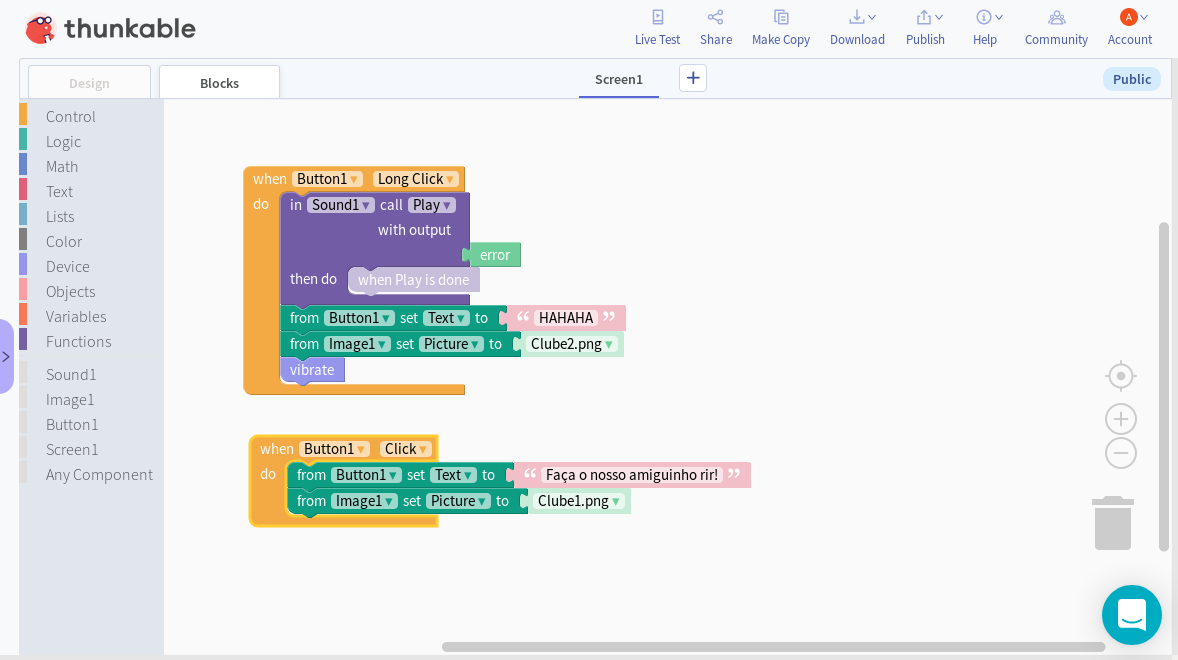
\includegraphics[width=0.9\textwidth]{GuiaThunk1Blocks.png}
    \caption{Tela Design}\label{fig:telablocks}
\end{figure}

Por exemplo, decida quantas vezes você quer que uma ação se repita, quando a ação deve acontecer, etc. Para isso, arraste os blocos disponíveis na coluna da esquerda para a área de trabalho central, respeitando o formato de encaixe entre blocos. Aponte sobre um bloco com o mouse para ver informações sobre este bloco. Você pode remover blocos usando o teclado (tecla Delete) ou arrastando o bloco para a lixeira, no canto inferior direito da tela.

Observe que, para cada componente inserido na tela, há um conjunto de blocos relacionados a ele. Os blocos irão ordenar uma ação específica sobre o componente (por exemplo, o que ocorrerá ao apertar um botão). Note que há várias formas de organizar os blocos para fazer uma mesma ação (que tal tentar usar o mínimo de blocos possível?).

Enfim, na tela Blocks, você estará trabalhando com a lógica computacional, por isso: \textbf{arrisque-se!}

%----------------------------------------------------------------------------------------
%	CHAPTER 2
%----------------------------------------------------------------------------------------
\chapterimage{Capa2.png} % Chapter heading image

\chapter{Meus primeiros aplicativos}

\section{Primeiro aplicativo: Faça cócegas no personagem!}\index{App1}

Nosso primeiro aplicativo vai exibir a imagem de um personagem e um botão que, quando pressionado por um tempo, fará o personagem mudar de aparência e dar risada (Figura \ref{fig:primeiroapp}). É um aplicativo simples para você fazer cócegas no personagem!


\begin{figure}[H]
	\centering

    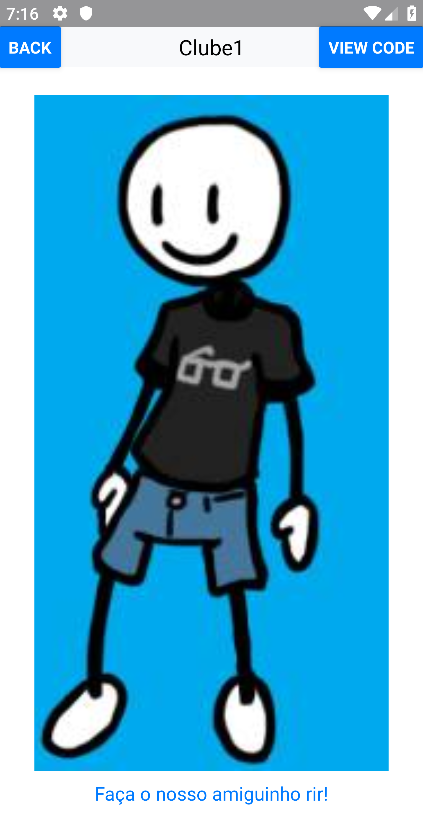
\includegraphics[width=0.35\textwidth]{GuiaThunkClube1Tela1.png}\hspace{0.2cm}
    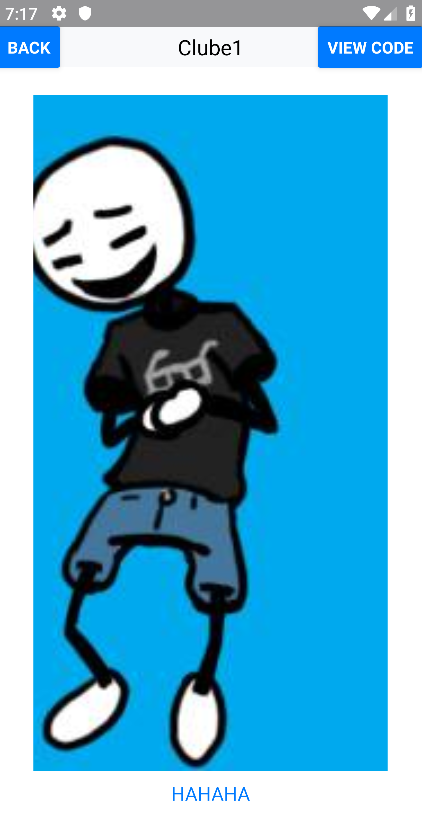
\includegraphics[width=0.35\textwidth]{GuiaThunkClube1Tela2.png}
	\caption{Primeiro aplicativo}\label{fig:primeiroapp}
\end{figure}

Para começar, como mostrado no capítulo~\ref{ch:thunkable}, acesse o site do Thunkable e comece um novo projeto, dando a ele o nome de Clube1.

\subsection{Adicionando arquivos no projeto}

Precisaremos de três aquivos -- duas imagens e um arquivo de som -- que encontram-se neste endereço:
 \url{http://bit.ly/clube1thunk}

Faça download de cada um dos arquivos e salve-os em uma pasta no seu computador. Agora vamos voltar para o Thunkable e começar construir a tela (Screen1) do aplicativo. 




Na estrutura do aplicativo (área superior à esquerda), encontre a seção ``Files'' e clique em ``Choose a File'' para adicionar ao projeto os arquivos que você recém baixou para seu computador (Figura \ref{fig:upload}).
Caso esta seção não esteja aparecendo, use o mouse para movimentar a barra de rolagem para baixo e assim visualizar mais itens. Quando você clicar em ``Choose a File'', aparecerá uma tela para você selecionar arquivos a serem incorporados ao projeto. Selecione os arquivos Clube1.png, Clube2.png e risada.mp3 e envie-os ao projeto. Veja que esses arquivos aparecem listados na área de arquivos (Files) da tela Screen1. 

\begin{figure}[H]
 	\centering   
	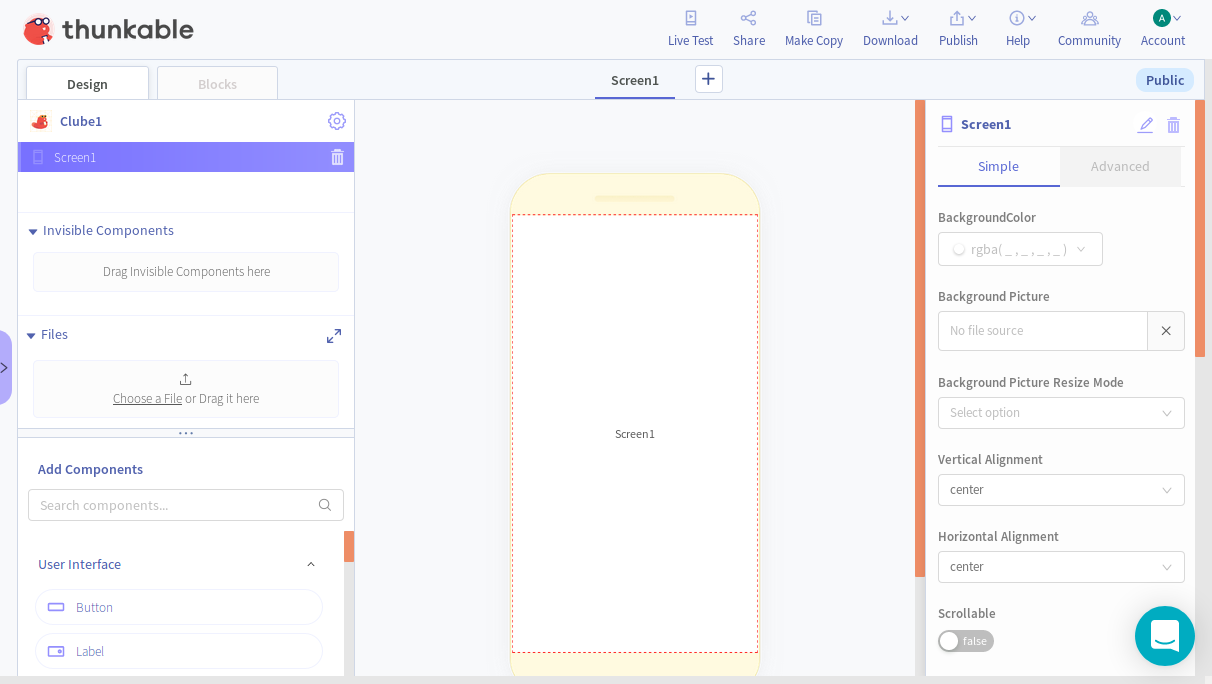
\includegraphics[width=0.9\textwidth]{GuiaThunkUpload.png}
    \caption{Enviando arquivos ao projeto}\label{fig:upload}
\end{figure}

\subsection{Criando a tela do aplicativo}

Agora vamos adicionar à tela (Screen1) os componentes necessários para o nosso aplicativo: uma imagem (Image), um botão (Button) e um som (Sound). 
\begin{enumerate}
\item Use a caixa de busca ou a barra de rolagem em ``\textbf{Add Components}'' para localizar cada componente, depois arraste-o para a tela do aplicativo. Veja que a lista de componentes do projeto também é atualizada à medida que você insere componentes na tela.
\item É hora de editar os componentes inseridos para alterar as propriedades de cada um. Para isso, você deverá clicar no componente e configurar as propriedades na \textbf{área de propriedades à direita na tela Design} do projeto:

	\begin{enumerate}[label=(\alph*)]
    	\item No componente Image1, clique em Picture e selecione a imagem Clube1.png. Depois, ajuste a altura da imagem (Height) escolhendo ``Pick One: Fit contents, Fill container'' e logo abaixo ``Fill Container''. Ajuste também a largura (Width), escolhendo ``Pick One: Fit contents, Fill container'' e logo abaixo ``Fill contents''. Estas propriedades fazem com que a imagem se ajuste ao tamanho da tela;
    	\item No componente Button1, altere a propriedade Text, digitando o texto ``Faça o nosso amiguinho rir!'';
    	\item No componente Sound1, clique em Source e selecione o arquivo risada.mp3.


	\end{enumerate} 

\item Além desses ajustes, você pode fazer outras edições da maneira que preferir, mudando o tamanho da fonte da legenda, as cores dos componentes, etc.
\end{enumerate}

\begin{figure}[H]
 	\centering   
	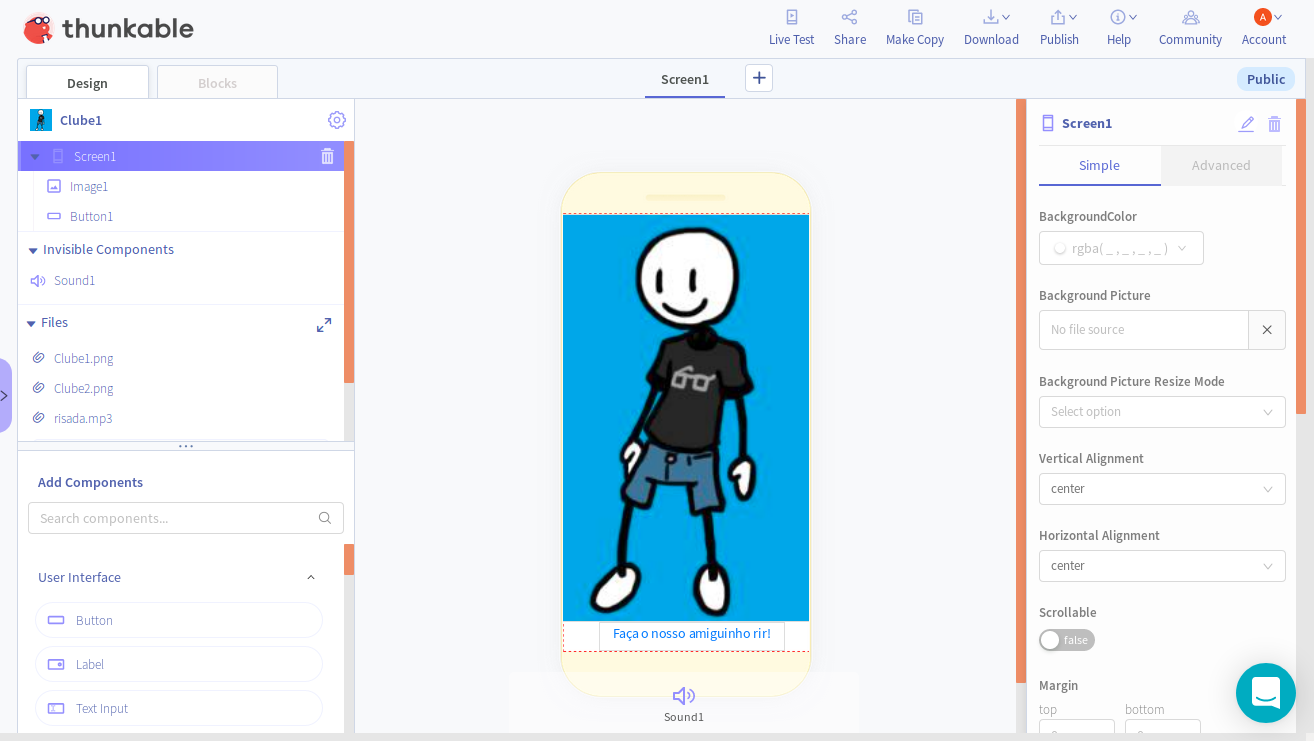
\includegraphics[width=0.8\textwidth]{GuiaThunkClube1Design.png}
    \caption{Enviando arquivos ao projeto}\label{fig:clube1design}
\end{figure}
	
	
\subsection{Programando os blocos do aplicativo}


E finalmente... vamos aos blocos! Para isso, clique na aba Blocks. No menu à esquerda, clique em Button1. Observe que há um conjunto de blocos diretamente relacionado a este componente, que é da categoria Button (Figura \ref{fig:clube1blocks1}). Vamos precisar desses blocos para programar o aplicativo.

\begin{figure}[H]
	\centering
    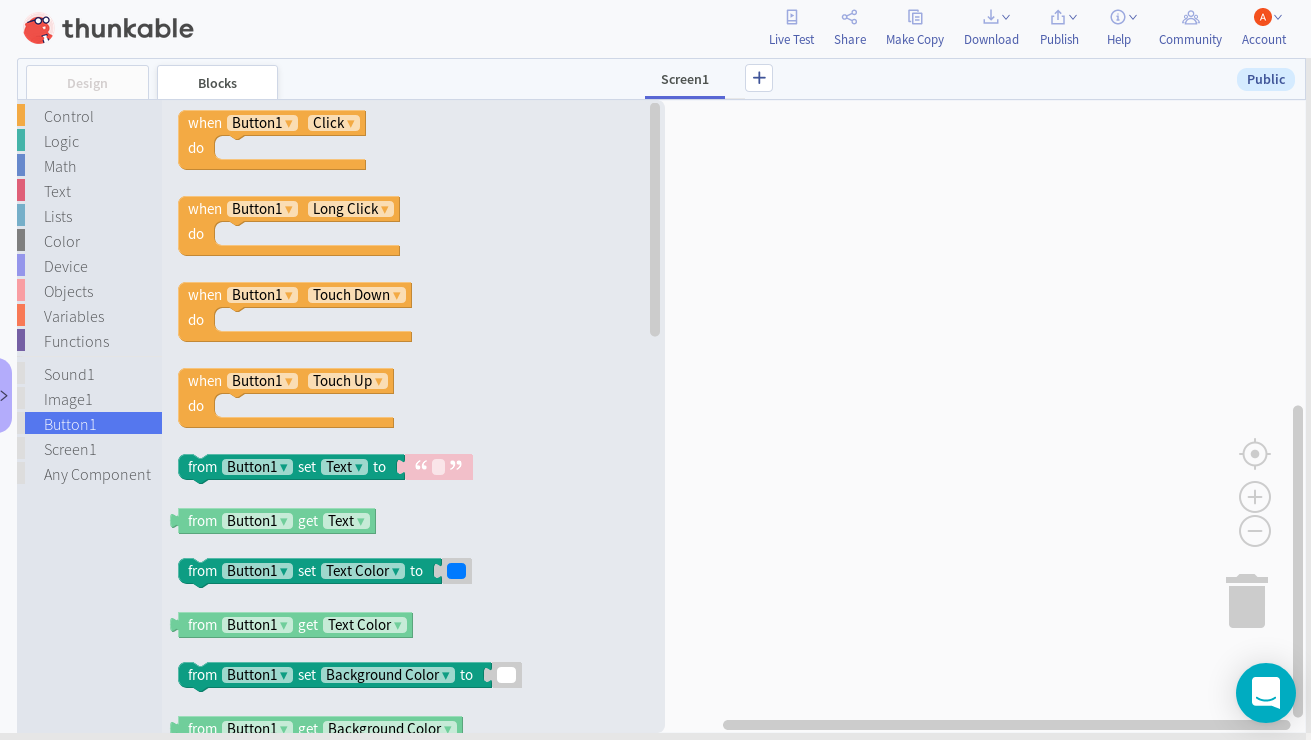
\includegraphics[width=0.65\textwidth]{GuiaThunkClube1Blocks1.png}
    \label{fig:clube1blocks1}
    \caption{Blocos relacionados ao componente da categoria Button}
\end{figure}

Para completar nosso primeiro aplicativo, siga estes passos:

\begin{enumerate}

%	\begin{enumerate}[label=(\alph*)]
	\item Selecione Button1 para ver os blocos de programação deste componente. Arraste o bloco ``when Button1 Long Click do'' para a área de blocos. Este bloco servirá para programarmos o que acontecerá quando o botão for pressionado durante um tempo:  o personagem vai dar risada, o botão vai mostrar outro texto, a imagem vai ser substituída e o celular vai vibrar.
	\item Para que o personagem dê risada, clique em Sound1 e arraste o bloco ``in Sound1 call Play'';
	\item Para que o botão seja modificado, clique em Button1 e arraste o bloco ``from Button1 set Text to ``''''. Clique entre as aspas e digite o texto HAHAHA;
	\item Para que a imagem seja substituída, clique em Image1 e arraste o bloco ``from Image1 set Picture to Clube1.png''. Clique no nome do arquivo (Clube1.png) e selecione outra imagem (Clube2.png);
	\item Para adicionar uma vibração no celular, clique em Device (dispositivo) e arraste o bloco ``vibrate''.


\end{enumerate}

Ao final desta parte, você terá os blocos organizados conforme mostra a Figura \ref{fig:clube1blocks2}.

\begin{figure}[H]
	\centering
    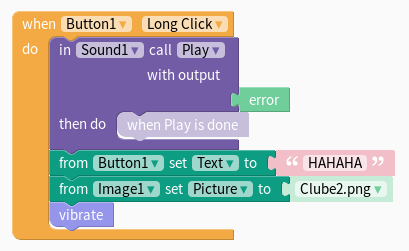
\includegraphics[width=0.6\textwidth]{GuiaThunkClube1Blocks2.png}
     \caption{Blocos do primeiro aplicativo}\label{fig:clube1blocks2}
   
\end{figure}


E assim concluímos a criação do projeto Clube1! Você pode verificar como ficou o seu aplicativo seguindo as instruções do capítulo ~\ref{ch:teste}.

Você pode incrementar ainda mais seu aplicativo, fazendo o personagem voltar ao normal quando o botão for clicado rapidamente. Para isso, arraste o bloco ``when Button1 Click do'' para a área de blocos e preencha-o com 2 blocos, para configurar o botão e a imagem de volta ao estado inicial. Dica: os blocos são os mesmos usados anteriormente, só que preenchidos com texto e arquivo iniciais. A Figura \ref{fig:clube1blocks3} ilustra como ficarão os blocos adicionais.


\begin{figure}[H]
	\centering
    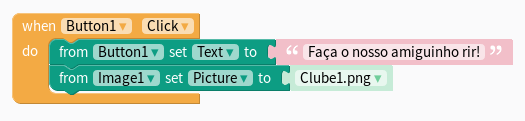
\includegraphics[width=0.7\textwidth]{GuiaThunkClube1Blocks3.png}
    \caption{Blocos adicionais para incrementar o primeiro aplicativo}\label{fig:clube1blocks3}
    
\end{figure}

%----------------------------------------------------------------------------------------

\section{Segundo aplicativo: Cálculo do IMC}\index{App2}

Agora vamos criar um aplicativo para o cálculo do IMC (Índice de Massa Corporal). Nele, o usuário insere o seu peso e a sua altura e o aplicativo retorna uma classificação de acordo com o IMC calculado (peso normal, sobrepeso, etc.). Além disso, pode-se saber mais sobre o cálculo clicando no botão de ``Informações''.

Para este aplicativo, crie um novo projeto no Thunkable com o nome de Clube2. 

\subsection{Adicionando arquivo no projeto}

Para este projeto, precisaremos de 1 imagem que pode ser baixada neste link:
\url{http://bit.ly/clube2thunk}
%\url{https://drive.google.com/file/d/0B6vOtDABI918VE4zbGR2cVdCTmc/view?usp=sharing}


\subsection{Criando as telas do aplicativo}


Neste projeto, vamos usar 2 telas, conforme mostra a Figura \ref{fig:telasimc}. Os componentes necessários para cada uma são os seguintes:

\begin{figure}[H]
	\centering
    %\includegraphics[width=0.45\textwidth]{GuiaApp53.png}\hspace{0.2cm}
    %\includegraphics[width=0.45\textwidth]{GuiaApp54.png}
    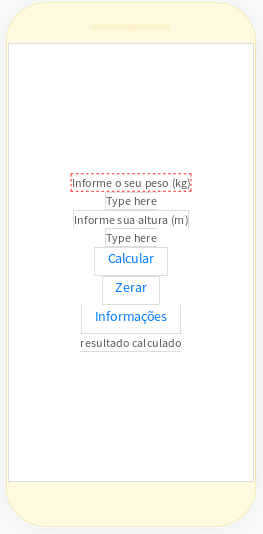
\includegraphics[width=0.35\textwidth]{GuiaThunk2TelaIMC1.png}\hspace{0.2cm}
    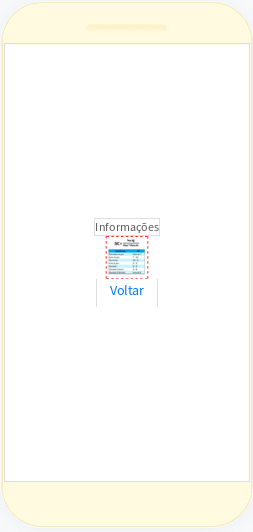
\includegraphics[width=0.34\textwidth]{GuiaThunk2TelaIMC2.png}
	\caption{Telas do aplicativo de cálculo do IMC}\label{fig:telasimc}
\end{figure}

\begin{description}
    \item[Screen1:] Nesta tela, vamos usar 3 componentes do tipo Label (textos fixos) para escrever textos na tela: ``Informe o seu peso (kg)'', ``Informe sua altura (m)'' e o resultado do cálculo. Também vamos usar 3 componentes Button (botões), para Calcular, Zerar e mostrar Informações. Para o usuário poder digitar seus dados, vamos adicionar 2 caixas de entrada de texto (Text input). Para posicionar os componentes na ordem certa, arraste-os para dentro da estrutura do aplicativo e preste atenção às linha que aparece indicando a posição de inserção. Inicialmente, vamos deixar a aparência padrão dos componentes. Mais tarde você poderá ajustá-los melhor. A aparência inicial desta tela é mostrada na primeira coluna Figura \ref{fig:telasimc}.
    
    \item[Screen2:] Na segunda tela, vamos usar um componente Label com o texto ``Informações'', uma imagem (Image) e um Button com o texto ``Voltar''. Na imagem, selecione o arquivo com imagem sobre o cálculo do IMC, baixado no início da criação do projeto. A aparência inicial desta tela é mostrada na segunda coluna da Figura \ref{fig:telasimc}. Novamente, não se preocupe por enquanto com o ajuste da aparência.
    
\end{description}




\subsection{Programando os blocos do aplicativo}

Neste projeto, vamos usar diferentes tipos de blocos que vão ser ativados quando o usuário clicar em cada botão. A parte mais importante da lógica do aplicativo é o cálculo do IMC. Para realizar este cálculo, vamos usar os dados informados pelo usuário e vamos armazenar o resultado em uma \textbf{variável}.

Na tela Blocks, veja que existe a seção Variables, onde ficam os blocos que manipulam variáveis. Para utilizar uma variável, você deve inicializá-la com um valor e dar um nome a ela. Essa irá se chamar ``imc'' e vai armazenar o resultado do cálculo do IMC, utilizando os valores de peso e altura digitados pelo usuário (Figura \ref{fig:imcvar}).

\begin{figure}[H]
	\centering
	%\includegraphics[width=\textwidth]{GuiaApp55.png}\hspace{0.2cm}
	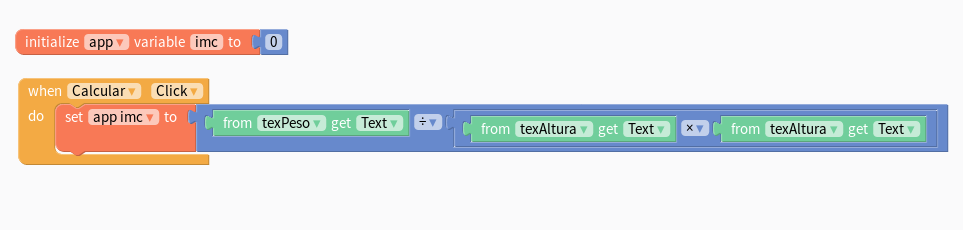
\includegraphics[width=\textwidth]{GuiaThunk2Var.png}\hspace{0.2cm}
	\caption{Blocos de inicialização e alteração da variável para cálculo do IMC}\label{fig:imcvar}
\end{figure} 

Com o valor do IMC calculado, vamos compará-lo com os valores da tabela da imagem baixada, para obter uma classificação sobre o peso do usuário. Para isso, precisaremos de um bloco da seção Control: o bloco de controle condicional ``if... else...''. Esse bloco será usado para comparar o valor da variável "imc" com o valor de cada classificação da tabela até encontrar a classificação adequada, que será escrita no Label destinado a apresentar a resposta. A Figura \ref{fig:imcifs} ilustra o estado final do bloco executado para o botão ``Calcular'', incluindo o bloco condicional e todos os testes de condições que o compõem.

\begin{figure}[H]
	\centering
	%\includegraphics[width=\textwidth]{GuiaApp56.png}\hspace{0.2cm}
	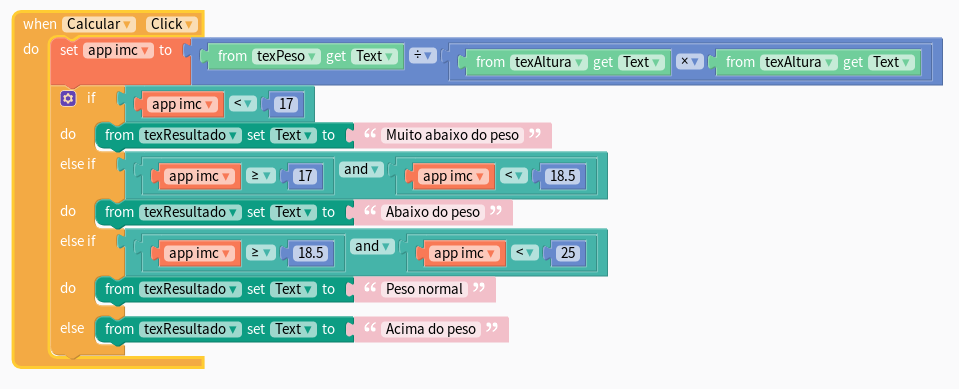
\includegraphics[width=\textwidth]{GuiaThunk2Calcular.png}\hspace{0.2cm}
    \caption{Blocos executados para o botão ``Calcular''}\label{fig:imcifs}

\end{figure} 

Por fim, vamos controlar o que os outros botões fazem. Quando o botão de ``Zerar'' for clicado, os valores inseridos deverão ser apagados para que novos valores possam ser calculados. Quando o botão ``Informações'' for clicado, iremos para a segunda tela (Screen2).

\begin{figure}[H]
	\centering
	%\includegraphics[width=\textwidth]{GuiaApp57.png}\hspace{0.2cm}
	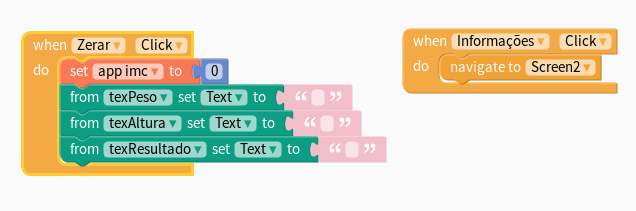
\includegraphics[width=\textwidth]{GuiaThunk2Zerar.png}\hspace{0.2cm}
    \caption{Blocos para os botões ``Zerar'' e ``Informações''}\label{fig:imczerar}
\end{figure} 



Nesta segunda tela, apenas precisaremos nos preocupar com o botão ``Voltar'', que, ao ser clicado, deve retornar para a primeira tela (Screen1).
 
\begin{figure}[H]
	\centering
	%\includegraphics[width=\textwidth]{GuiaApp57.png}\hspace{0.2cm}
	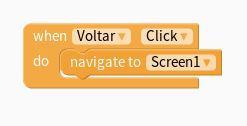
\includegraphics[width=0.4\textwidth]{GuiaThunk2Voltar.png}\hspace{0.2cm}
    \caption{Blocos para o botão ``Voltar'' da segunda tela}\label{fig:imcvoltar}
\end{figure} 

 
E assim concluímos a criação do projeto Clube2! Você pode verificar como ficou o seu aplicativo seguindo as instruções do capítulo ~\ref{ch:teste}. Se você quiser incrementar ainda mais seu aplicativo, siga as dicas da próxima seção!


\subsection{Incrementando o visual do seu aplicativo}

As telas do seu aplicativo podem ficar mais interessantes se você ajustar as propriedades de cada componente. Na Figura \ref{fig:imcmelhor} está um exemplo de como pode ficar sua primeira tela (Screen1).

\begin{figure}[H]
	\centering
	%\includegraphics[width=\textwidth]{GuiaApp57.png}\hspace{0.2cm}
	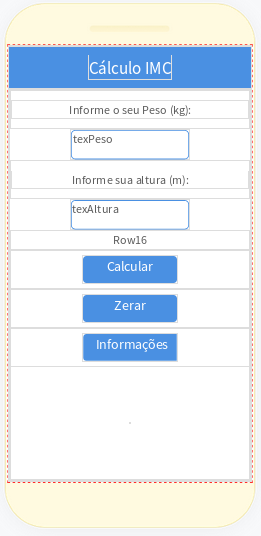
\includegraphics[width=0.3\textwidth]{GuiaThunk2Melhorado.png}\hspace{0.2cm}
    \caption{Novo visual para a primeira tela}\label{fig:imcmelhor}
\end{figure} 

Para obter este visual, você pode:

\begin{itemize}
    \item usar os componentes Row e Column, que permitem organizar o layout do aplicativo em linhas e colunas (no caso, 1 coluna e 9 linhas). Com isso, fica mais fácil ajustar espaçamentos entre os componentes;
    \item nas caixas de entrada de texto (Text input), ajustar a cor e o arredondamento da borda (border radius);
    \item nos botões, alterar a cor de fundo e a cor do texto.
\end{itemize}

%----------------------------------------------------------------------------------------
%	CHAPTER 3
%----------------------------------------------------------------------------------------
\chapterimage{Capa3.png} % Chapter heading image

%Bandeiras
%https://atlasescolar.ibge.gov.br/download-atlas

\chapter{Aplicativo Quiz}\label{ch:appquiz}

Neste capítulo, partiremos de um projeto já iniciado e explicaremos os componentes visuais e os blocos utilizados. O aplicativo escolhido é um Quiz sobre bandeiras de estados brasileiros. Mas... o que é um aplicativo Quiz?

\section{O que é o Flags Quiz?}


Um Quiz é basicamente um aplicativo de perguntas e respostas em formato de jogo. O objetivo do jogo é testar o conhecimento do jogador no assunto (ou tema) proposto. As respostas podem ser digitadas ou podem ser de múltipla escolha, e apenas uma resposta será a correta. O usuário vai acumulando pontos conforme for acertando as respostas. 

Nosso Quiz servirá para testar o conhecimento sobre bandeiras (e siglas) de estados brasileiros, por isso o título dele será ``Flags Quiz'' (em inglês, flag significa bandeira). O aplicativo de exemplo tem poucas questões e caberá a você acrescentar outras bandeiras ao Quiz!


O aplicativo está disponível neste link: \url{http://bit.ly/flagsthunk}.
%\url{https://x.thunkable.com/copy/ef6e95313d2bdfb9d1bc61b5d870ce3a}
Basta clicar no link para que o aplicativo seja adicionado aos seus projetos.

% Para começar, após ter feito o \textit{download} do arquivo Quiz.aia, acesse o site MIT App Inventor como de costume.
% Clique no menu \textit{Projetos} (1) e selecione a opção \textit{Importar projeto (.aia) do meu computador...}. Na janela que se abrirá, clique em \textit{Escolher arquivo} (2) e abra o arquivo “Quiz.aia” baixado anteriormente, termine clicando em \textit{Ok} (3).

% \begin{figure}[H]
%  	\centering
%     \includegraphics[width=0.77\textwidth]{GuiaApp7.png}
%     \label{fig:guia7}
% \end{figure}

\section{Tela Design}
Ao abrir o projeto, na tela Design (Figura \ref{fig:quizdesign}), é possível notar que os seguintes componentes:

\begin{enumerate}
\item Na primeira linha da tela (Row1), há 2 componentes do tipo Label. Um deles (Label1) tem o texto ``Pontos'' e o outro (LabelPontos) tem o texto ``0''. O LabelPontos será atualizado sempre que o jogador acertar uma questão. O Label1 se manterá fixo.
\item No centro da tela, temos uma coluna (Column1) com 3 componentes: um Label (Label2) contendo a pergunta ``Qual estado brasileiro tem esta bandeira?'', um componente Image (ImagemBandeira) e um componente Text Input (InputEstado), onde o usuário vai digitar usa resposta. A imagem será atualizada quando o usuário acertar uma resposta. A pergunta se manterá fixa.
\item No final da tela (Row2), há um componente do tipo Button (Button1). O usuário clicará nesse botão para enviar sua resposta. 

\end{enumerate}

\begin{figure}[H]
	\centering
	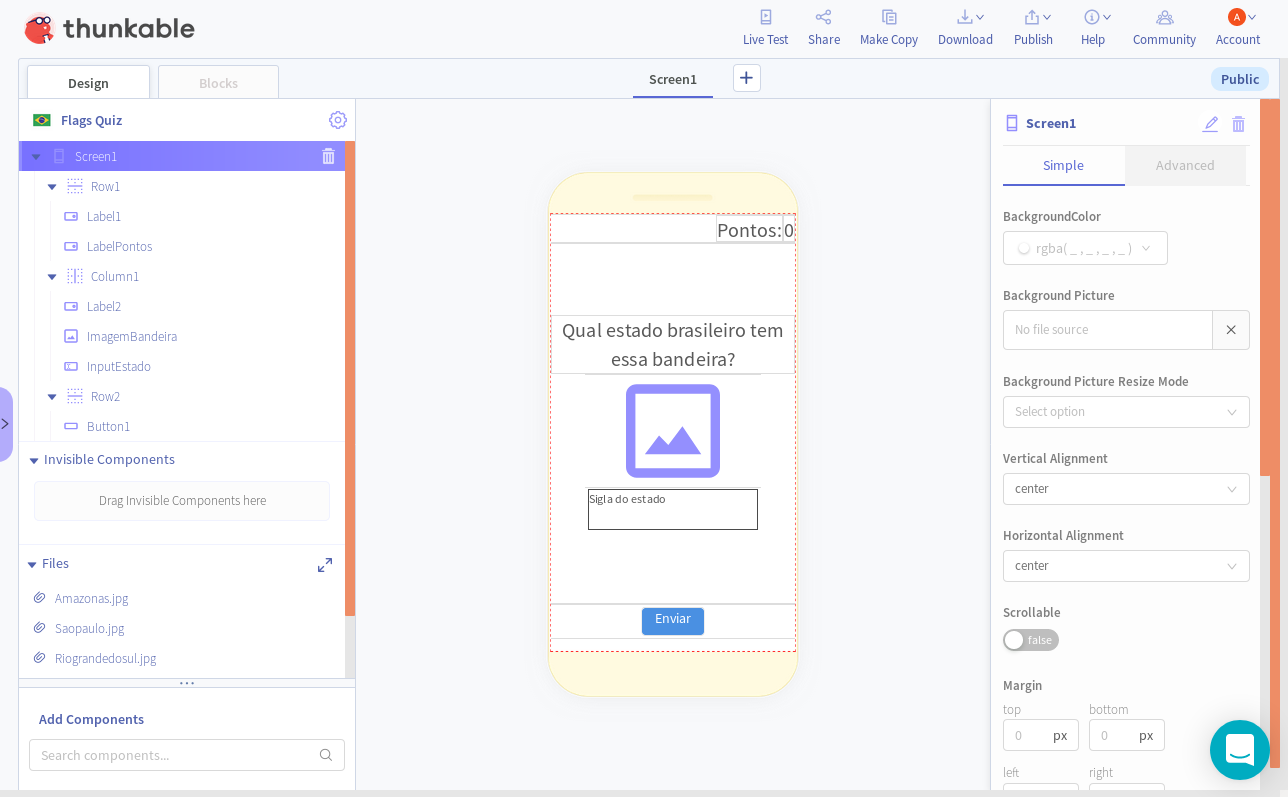
\includegraphics[width=0.9\textwidth]{GuiaThunkQuizDesign.png}\hspace{0.2cm}
    \caption{Tela Design do aplicativo Quiz}\label{fig:quizdesign}
\end{figure} 

Você deve estar se perguntando o que são os componentes do tipo Row e Column, pois eles não tinham sido usados nos exemplos anteriores. Tratam-se de componentes de Layout, que ajudam a dividir a tela em partes e assim posicionar melhor os demais componentes.

Observe também que o projeto tem 3 arquivos de bandeiras: Amazonas.jpg, Saopaulo.jpg e Riograndedosul.jpg. Você pode obter mais bandeiras em \url{https://atlasescolar.ibge.gov.br/images/atlas/bandeiras_brasil.zip}.


A princípio nada será alterado na área de ``Design'', portanto vamos ver o que temos na tela de blocos. 

\section{Tela Blocks}

Na tela de blocos, precisaremos de alguns conjuntos de blocos que explicaremos por partes a seguir.

\subsection{Variáveis do aplicativo}

No topo da tela de blocos, há dois pares de blocos bem semelhantes (Figura \ref{fig:quizvars}). Tratam-se de \textbf{variáveis}, que guardam dados importantes para o funcionamento do nosso aplicativo.

\begin{figure}[H]
	\centering
	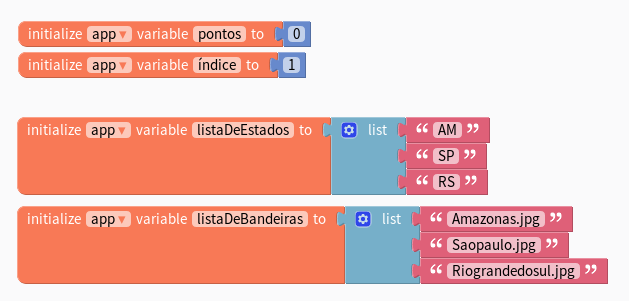
\includegraphics[width=0.7\textwidth]{GuiaThunkQuizVars.png}\hspace{0.2cm}
    \caption{Variáveis do aplicativo Quiz}\label{fig:quizvars}
\end{figure} 

Cada variável no nosso aplicativo tem um propósito:
\begin{itemize}
    \item A variável ``pontos'' tem o seu valor inicialmente em zero e, como seu próprio nome sugere, guardará a pontuação do usuário e terá seu valor incrementado em 1 para cada resposta correta. 
    \item A variável ``índice'' é responsável pelo controle das listas de bandeiras e de estados, que serão vistas a seguir. Esta variável tem o seu valor inicialmente em 1, mas esse valor será alterado (será sorteado um novo valor) quando o aplicativo iniciar.
    \item As variáveis ``listaDeEstados'' e ``listaDeBandeiras'' são variáveis que contêm conjuntos (listas) de valores. A primeira contém as siglas dos estados, que são as respostas esperadas para cada questão. A segunda contém a lista de bandeiras, isto é, nomes dos arquivos que contêm as imagens de bandeiras (arquivos que estão na seção Files da estrutura do aplicativo). Estes nomes serão usados mais adiante para configurar a imagem que será mostrada a cada vez.
    Note que o primeiro elemento da lista de estados corresponde ao primeiro elemento da lista de bandeiras, e o mesmo vale para os elementos seguintes. Essa correspondência é importante, pois nos permitirá usar a variável ``índice'' para escolher elementos correspondentes em cada lista.

\end{itemize}


 
\subsection{Controle da inicialização da tela}


Logo abaixo das variáveis, temos o bloco apresentado na Figura \ref{fig:quizstart}. Esse bloco controla a inicialização da tela do aplicativo (``when Screen1 Starts do'') e tem um pequeno conjunto de outros blocos em seu corpo. O conjunto de instruções dentro deste bloco será executado assim que a Screen1 do projeto, neste caso a única tela, for iniciada. Deste modo, podemos dizer que essas instruções serão executadas instantaneamente ao abrirmos o aplicativo.


\begin{figure}[H]
	\centering
	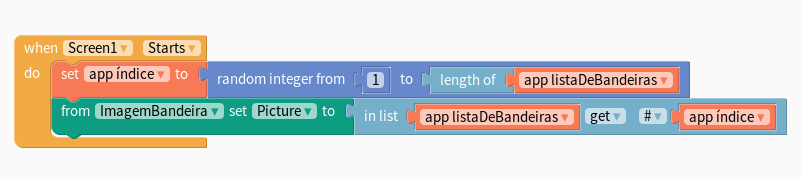
\includegraphics[width=0.7\textwidth]{GuiaThunkQuizStart.png}\hspace{0.2cm}
    \caption{Blocos de inicialização da tela aplicativo Quiz}\label{fig:quizstart}
\end{figure} 


	


Dentro deste bloco, as ações são as seguintes:
\begin{enumerate}
\item A variável ``índice'' tem seu valor ajustado para um valor sorteado entre 1 e 3, que é o tamanho (length) da lista de bandeiras. O bloco ``random integer from'', que faz parte da categoria de blocos de matemática (Math), é muito útil neste ponto. No entanto, note que um sorteio entre apenas 3 números pode facilmente repetir valores. Se, em vez de sortear um número, você desejasse começar com o primeiro item da lista, você poderia remover este bloco, deixando o índice com o valor inicial.
\item A imagem ``ImagemBandeira'' é ajustada de forma a mostrar o elemento (arquivo) da lista de bandeiras correspondente ao índice sorteado. Assim, se for sorteado o índice 3, será mostrado o arquivo Riograndedosul.jpg (bandeira do RS), que é o terceiro elemento da lista.

\end{enumerate}

\subsection{Controle do botão}

Na última parte da tela de blocos (Figura \ref{fig:quizbutton}), temos o bloco que controla o que acontece quando o botão é clicado (``when Button1 Click''). Em outras palavras, este bloco trata o evento 'Click' no botão. 

\begin{figure}[H]
	\centering
	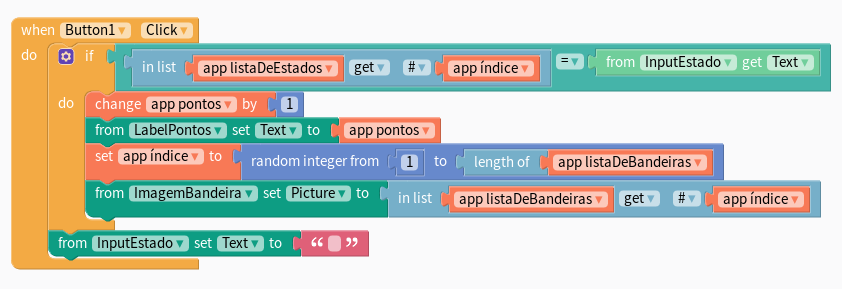
\includegraphics[width=\textwidth]{GuiaThunkQuizButton.png}\hspace{0.2cm}
    \caption{Programação do botáo do aplicativo Quiz}\label{fig:quizbutton}
\end{figure} 


Dentro deste bloco, temos um bloco de \textbf{controle condicional} (``if .. do'' ou ``se .. faça''), que vai verificar se o jogador acertou a resposta e, em caso positivo, ajustar a tela do aplicativo. Mais detalhadamente, temos o seguinte:
\begin{itemize}
    \item Condição: se o texto digitado pelo usuário (``from InputEstado get Text'') for igual ao item de número ``índice'' da lista de estados, faça
    \item Atualiza pontuação: o bloco ``change app pontos by 1'' faz a variável ``pontos'' ser incrementada e o bloco ``from LabelPontos set Text to app pontos'' faz o Label correspondente ser atualizado na tela, mostrando o novo valor da variável ``pontos''.
    \item Sorteia nova questão: os 2 últimos blocos dentro do ``if .. do'' são os mesmos usados na inicialização para sortear a questão, ou seja, configurar os novos valores para a variável ``índice'' e  para ``ImagemBandeira''.
\end{itemize}

Ainda dentro do bloco que trata o evento Click no botão, temos um último bloco que é executado incondicionalmente.  Esse bloco apenas ``limpa'' o texto digitado pelo usuário, ou seja, coloca um texto vazio em ``InputEstado''.



%----------------------------------------------------------------------------------------
%	CHAPTER 5
%----------------------------------------------------------------------------------------
\chapterimage{Capa5.png}

\chapter{Testando seu aplicativo}\label{ch:teste}

Após ter criado o seu aplicativo, ou enquanto o desenvolve, você vai querer testá-lo, não é mesmo? Para isso, você vai precisar instalar um aplicativo chamado Thunkable Live no seu smartphone. Ele está disponível nas lojas de aplicativos para Android (Figura \ref{fig:live}) ou iPhone.




\begin{figure}[H]
	\centering
    %\includegraphics[width=0.65\textwidth]{GuiaApp28.png}
    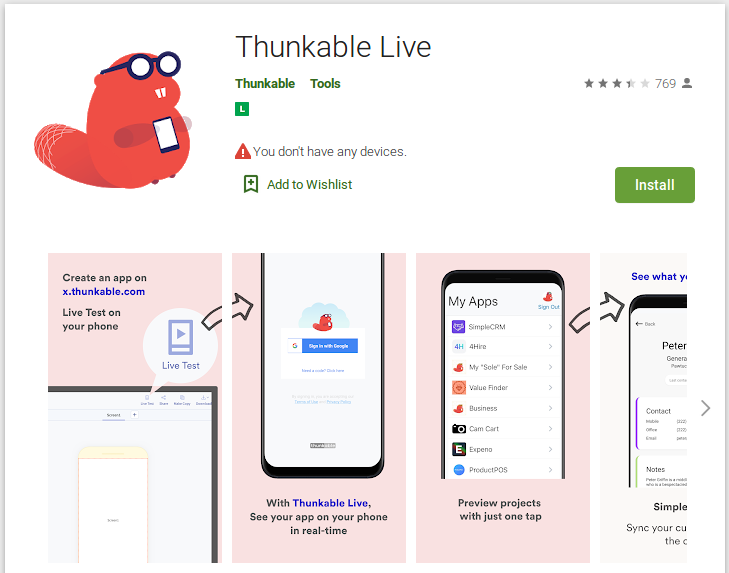
\includegraphics[width=0.7\textwidth]{GuiaThunk5Live.png}
    \caption{Aplicativo Thunkable Live na Play Store}\label{fig:live}
\end{figure}

Depois de baixar o aplicativo Thunkable Live, você deverá abri-lo e entrar com a mesma conta de e-mail que está sendo usada no site do Thunkable para criar seus projetos.

Na tela do aplicativo Thunkable Live, você verá a lista de seus projetos (Figura \ref{fig:livetest}). Para testar um projeto, basta clicar sobre ele.

\begin{figure}[H]
	\centering
    %\includegraphics[width=0.65\textwidth]{GuiaApp28.png}
    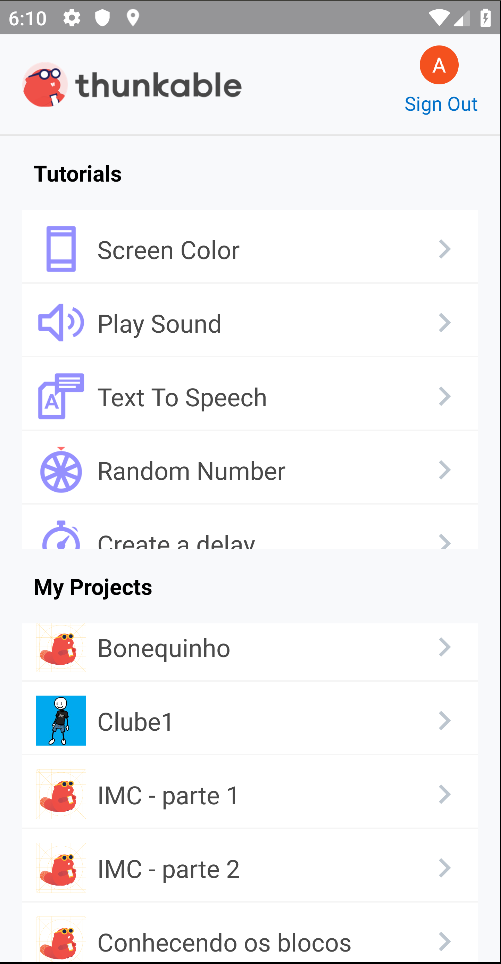
\includegraphics[width=0.3\textwidth]{GuiaThunk5LiveTest.png}
    \includegraphics[width=0.305\textwidth]{GuiaThunk5LiveIMC.png}

    \caption{Lista de projetos no aplicativo Thunkable Live e teste de um projeto}\label{fig:livetest}
\end{figure}


%----------------------------------------------------------------------------------------
%	CHAPTER 4
%----------------------------------------------------------------------------------------
\chapterimage{Capa4.png}

\chapter{Conhecendo melhor os blocos}

À primeira vista, pode parecer complicado entender todos os blocos e suas funcionalidades. Porém, todos eles funcionam sobre ideias muito simples, que são combinadas para compor cada aplicativo .

Na lateral esquerda da área de blocos (aba Blocks), podemos ver o \textbf{menu} que organiza os blocos rm \textbf{categorias} (Figura \ref{fig:menublocos}):

\begin{figure}[H]
	\centering
	\includegraphics[width=0.45\textwidth]{GuiaThunk4Blocos.png}
    \caption{Menu de blocos organizados por categorias}\label{fig:menublocos}	
\end{figure}

%----------------------------------------------------------------------------------------

\section{Blocos de Controle Condicional}\index{Controle}

%\begin{quote}
\begin{minipage}{0.35\textwidth}
	\includegraphics[width=\linewidth]{GuiaThunk4Cond1.png}
	\includegraphics[width=\linewidth]{GuiaThunk4Cond2.png}
\end{minipage}
\hfill
\begin{minipage}{0.6\textwidth}\raggedright
	Na categoria \textbf{Control} estão vários blocos que controlam a lógica de funcionamento do aplicativo. Aqui vamos nos concentrar no bloco de controle condicional (bloco \textbf{if}), que serve basicamente para executar uma ação \textbf{se} uma condição for satisfeita. Este bloco nunca é usado sozinho: você vai precisar preenchê-lo com pelo menos 2 outros blocos: (a) um bloco \textbf{lógico}, que representa a condição a ser testada e que deverá resultar em verdadeiro ou falso, e (b) um bloco que representa a ação. O bloco \textbf{if} também tem outros sub-blocos de controle: o bloco \textbf{else if}, que serve para testar outra condição caso a anterior não tenha sido satisfeita, e o bloco \textbf{else}, que serve para indicar a ação a ser executada quando nenhuma condição for satisfeita.
	
\end{minipage}
%\end{quote}

%----------------------------------------------------------------------------------------

\section{Blocos de Lógica}\index{Logica}

%\begin{quote}
\begin{minipage}{0.35\textwidth}
	\includegraphics[width=\linewidth]{GuiaThunk4Logic1.png}
	\includegraphics[width=\linewidth]{GuiaThunk4Logic2.png}
\end{minipage}
\hfill
\begin{minipage}{0.6\textwidth}\raggedright
	Na categoria \textbf{Logic}  estão os blocos de lógica, que representam uma condição que será testada. O resultado pode ser verdadeiro (\textbf{true}) ou falso (\textbf{false}). Os blocos de lógica mais comumente usados têm duas lacunas a serem preenchidas e um operador a ser selecionado. Por exemplo, o bloco lógico ``='' verifica a igualdade entre 2 blocos preenchidos à esquerda e à direita. Clicando-se no operador ``='', é possível trocá-lo por outro, por exemplo ``>''. Os blocos lógicos ``and'' e ``or'' comparam 2 blocos condicionais que podem	ser verdadeiros ou falsos. Por exemplo, você pode encaixar 2 blocos ``='' nas lacunas à esquerda e à direita de um bloco ``ou''. Se uma, ou ambas, as condições de igualdade forem verdadeiras, o bloco ``or'' resultará \textbf{true} , senão será \textbf{false}.
\end{minipage}
%\end{quote}

%----------------------------------------------------------------------------------------

\section{Blocos de Matemática}\index{Matematica}

%\begin{quote}
\begin{minipage}{0.35\textwidth}
	\includegraphics[width=\linewidth]{GuiaThunk4Math.png}
\end{minipage}
\hfill
\begin{minipage}{0.6\textwidth}\raggedright
	Na categoria \textbf{Math}, estão os blocos que fazem o aplicativo
	executar operações aritméticas, por exemplo multiplicação ou adição. Os operandos devem ser encaixados dentro dos blocos.
\end{minipage}
%\end{quote}

%----------------------------------------------------------------------------------------

\section{Blocos de Texto}\index{Texto}

%\begin{quote}
\begin{minipage}{0.45\textwidth}
	\includegraphics[width=\linewidth]{GuiaThunk4Text.png}
\end{minipage}
\hfill
\begin{minipage}{0.5\textwidth}\raggedright
	Na categoria \textbf{Text} estão os blocos que podem conter textos e realizar operações sobre eles, por exemplo: compará-los, alternar para minúsculo/maiúsculo,
	realizar buscas de palavras em um texto, dividir um texto, descobrir o tamanho em caracteres de um texto, etc. São blocos fundamentais para o
	aplicativo, e o seu uso permite a apresentação de informações nos componentes da tela.
\end{minipage}
%\end{quote}

%----------------------------------------------------------------------------------------

\section{Blocos de Listas}\index{Listas}
%\section{Blocos de Listas + EscolheLista}\index{Listas}

%\begin{quote}
\begin{minipage}{0.4\textwidth}
	\includegraphics[width=\linewidth]{GuiaThunk4List.png}
\end{minipage}
\hfill
\begin{minipage}{0.5\textwidth}\raggedright
	Na categoria \textbf{Lists} estão blocos que representam listas, isto é, conjuntos de dados. Listas servem para armazenar dados usados no aplicativo, que podem ser números, blocos de texto ou até mesmo componentes da tela.
	
% 	Um \textbf{EscolheLista} é um elemento visual de
% 	lista para a tela do app que pode ser
% 	colocado na tela através da aba de Design.
% 	Você pode escolher uma lista criada anteriormente
% 	para representar os elementos deste
% 	EscolheLista através do bloco "ajustar
% 	EscolheLista1.Elementos para", encaixando
% 	um bloco para \textbf{obter} a lista desejada.
\end{minipage}
%\end{quote}


%----------------------------------------------------------------------------------------

\section{Blocos de Variáveis}\index{Variaveis}

%\begin{quote}
\begin{minipage}{0.5\textwidth}
	\includegraphics[width=\linewidth]{GuiaThunk4Var.png}
\end{minipage}
\hfill
\begin{minipage}{0.45\textwidth}\raggedright
	Na categoria \textbf{Variables} estão blocos que servem para guardar dados úteis para seu aplicativo. Os dados podem ser mostrados ou alterados conforme a lógica do aplicativo. Toda variável deve receber um nome para que possa ser usada junto a outros blocos.
	Por padrão, variáveis são guardadas no próprio aplicativo (``app variable''), mas também podem ser armazenadas no dispositivo (``stored variable''), para que fiquem salvas quando o aplicativo for fechado.
	O bloco \textbf{initialize} serve para definir um valor
	inicial para uma variável. Para redefinir o valor do dado
	contido na variável, usa-se o bloco \textbf{set}. 
	%Para obter
	%o dado definido em uma variável, usa-se o bloco "obter".
	%Cada variável criada possui blocos de "ajustar" e "obter".
\end{minipage}
%\end{quote}

%----------------------------------------------------------------------------------------

\section{Blocos de Eventos}\index{Eventos}

%\begin{quote}
\begin{minipage}{0.5\textwidth}
	\includegraphics[width=\linewidth]{GuiaThunk4Event.png}
\end{minipage}
\hfill
\begin{minipage}{0.45\textwidth}\raggedright
	Os blocos de eventos servem para agrupar as ações que devem ser executadas quando (\textbf{when}) houver alguma ocorrência (evento) no aplicativo. Esses eventos referem-se,
	em geral, a interações com elementos da tela ou execução
	de alguns procedimentos previstos pelo aplicativo.
	Exemplos de eventos são os cliques (ou toques) em 
	componentes, abertura ou fechamento de uma tela, a
	ocorrência de um possível erro durante a execução, etc.
	Ao escolher um bloco de evento, você pode acoplar blocos
	em seu interior para definir o que acontecerá quando
	o evento acontecer. 
\end{minipage}
%\end{quote}

%----------------------------------------------------------------------------------------

\section{Blocos para Componentes Inseridos}\index{Objetos}

%\begin{quote}
\begin{minipage}{0.5\textwidth}
	\includegraphics[width=\linewidth]{GuiaThunk4Compo.png}
\end{minipage}
\hfill
\begin{minipage}{0.45\textwidth}\raggedright
	Os componentes adicionados
	na tela têm propriedades como texto, tamanho,
	cor, estado (ativo ou inativo), etc. Há propriedades que podem ser ajustadas na área de Design, mas também é possível usar blocos que fazem o ajuste. Para localizar esses blocos, você deve escolher o componente na lateral esquerda da área de Blocks. Os blocos de cor verde claro ou escuro ajustam propriedades do componente. Os blocos \textbf{from .. set} (verde escuro) alteram o valor de uma propriedade, enquanto os blocos \textbf{from ... get} (verde claro) obtêm a propriedade escolhida. Você pode encaixar esses blocos em blocos lógicos
	ou aritméticos para testes ou contas, por exemplo.
	\end{minipage}
%\end{quote}

%----------------------------------------------------------------------------------------
%	CHAPTER 6
%----------------------------------------------------------------------------------------
\chapterimage{Capa6.png}

\chapter{Programando mais aplicativos}\label{ch:mais}

\section{Um novo Quiz}

Agora que você já viu vários exemplos e já aprendeu mais sobre os blocos, que tal criar desde o início um novo aplicativo Quiz?  Nossa sugestão é que você crie um Quiz de perguntas e respostas com um tema à sua escolha. Você não precisa usar imagens, apenas os textos de perguntas e respostas. Para facilitar, escolha perguntas que possam ser respondidas com uma palavra, pois lembre que a ``correção'' é feita comparando a resposta esperada com a resposta digitada pelo jogador.

\begin{figure}[H]
	\centering
    %\includegraphics[width=\textwidth]{GuiaApp35.png}
    \includegraphics[width=\textwidth]{Pictures/GuiaThunkExtraQuizDesign.png}
    \caption{Sugestão de visual do novo aplicativo Quiz}\label{fig:extraquizdesign}
    \label{fig:guia35}
\end{figure}

Comece criando um novo projeto e dê um nome a ele, por exemplo ``Extra Quiz''. 
\subsection{Criando a tela do aplicativo}

Vamos precisar dos seguintes componentes na tela: 3 componentes do tipo Label, 1 Text Input e 1 Button. Além disso, use componentes Row para organizar o layout do aplicativo. A Figura \ref{fig:extraquizdesign} mostra uma sugestão de aparência da tela.


Quando você adicionar componentes que serão programados na tela Blocks, é importante dar \textbf{nomes significativos} a eles, pois assim ficará mais fácil de encontrá-los durante a programação. Por exemplo, se há mais de um Label, o Thunkable vai nomeá-los como Button1, Button2, etc., o que pode causar confusão. Você pode renomeá-los de forma a deixar mais claro o propósito de cada Label, por exemplo LabelPontos. 

Para \textbf{renomear} um componente, clique sobre ele para selecioná-lo e veja que seu nome aparece na área de propriedades à direita, na tela Design. Clique sobre o ícone que contém um lápis para ativar a edição do nome do componente e troque seu nome! Os componentes que sugerimos renomear neste projeto são os que serão manipulados durante o uso do aplicativo (e, por isso, durante a programação). A seguir está a lista desses componentes e os nomes sugeridos:

\begin{enumerate}
\item Label para mostrar a pontuação (LabelPontos);
\item Label que mostra a pergunta (LabelQuestão);
\item Text Input em que o jogador digita a resposta (InputResposta);
\item Button para enviar a resposta (ButtonEnviar).
\end{enumerate}

Já temos o básico que vamos precisar na tela inicial, então agora iremos construir a lógica para o funcionamento do app. Clique na aba Blocks e mãos à obra!

Assim como no Flags Quiz que apresentamos no capítulo \ref{ch:appquiz}, você pode dividir a programação deste aplicativo em 3 partes: as inicializações de variáveis, a inicialização da tela e o tratamento de evento no botão.

\subsection{Programando os blocos: variáveis}


Quanto às \textbf{variáveis}, vamos criar novamente as variáveis ``pontos'' e ``índice'', que foram usadas no Flags Quiz. Vamos também usar duas variáveis que guardam listas: ``listaDeQuestões'' e ``listaDeRespostas''. Abaixo detalhamos o passo a passo para programação desta parte:

\begin{enumerate}
    \item Para criar as variáveis ``pontos'' e ``índice'', clique na categoria \textbf{Variables} na coluna da esquerda da tela Blocks. Note que os blocos dessa seção têm a cor \textbf{laranja}. Arraste o bloco ``initialize app variable name to'' para a área central. Agora clique em ``name'' no bloco e digite o nome que você quer dar à sua variável (por exemplo, ``pontos''). Note que o bloco espera o encaixe de um outro bloco, que representa o valor que queremos guardar na variável. Neste caso, queremos um número, então vamos usar o primeiro bloco da categoria \textbf{Math}, que é um bloco bem simples com espaço para um número. Arraste este bloco para completar o bloco ``initialize app variable name to''. Para ajustar o valor, clique sobre ele e digite o número desejado. Você deverá repetir esses passos para cada uma das variáveis.
    \item Para criar as variáveis ``listaDeQuestões'' e ``listaDeRespostas'', inicialmente siga os mesmos passos das variáveis anteriores. No entanto, lembre que, em vez de guardar dados numéricos, estas variáveis vão conter conjuntos (listas) de dados textuais. Assim, não usaremos blocos da categoria Math, mas sim da categoria \textbf{Lists}. Clique nesta categoria e arraste o bloco ``list'' com 3 itens para a área central. Podemos desprezar os 3 itens numéricos: para isso, clique sobre cada um deles e tecle Delete/Del, ou ainda arraste-os para a lixeira. Agora vamos completar os valores dos itens da lista. Serão valores da categoria \textbf{Text}. Clique sobre esta categoria e arraste o bloco que contém aspas para dentro de um espaço livre no bloco ``list''. Você deverá repetir este procedimento para os demais itens das duas listas. Note que o primeiro item da lista de perguntas deverá corresponder ao primeiro item da lista de respostas, e assim por diante. Por exemplo, para a pergunta ``Qual é o maior país do mundo sem saída para o mar?'', deverá corresponder a resposta ``Cazaquistão''.
\end{enumerate}

Ao final desta parte, você deverá ter os blocos conforme mostra a Figura \ref{fig:extraquizvars}.


\begin{figure}[H]
	\centering
    \includegraphics[width=\textwidth]{Pictures/GuiaThunkExtraQuizVars.png}
    \caption{Variáveis do novo aplicativo Quiz}\label{fig:extraquizvars}
\end{figure}


Note que o bloco ``list'' permite que você ajuste a quantidade de itens da lista. Para isso, clique na pequena engrenagem branca sobre fundo azul no canto superior esquerdo do bloco ``list''. Você verá uma área de ``diálogo'' (como um balão de histórias em quadrinhos), dividida em duas partes (Figura \ref{fig:extraquizlist}). Na parte à esquerda, há o bloco ``item'', que pode ser movido para a parte à direita, dentro do bloco ``list'', para acrescentar itens à lista. Para remover um item da lista, clique sobre o item na parte à direita e mova-o para a esquerda.

\begin{figure}[H]
	\centering
    \includegraphics[width=0.6\textwidth]{Pictures/GuiaThunkExtraQuizList.png}
    \caption{Ajuste de elementos em um bloco ``list''}\label{fig:extraquizlist}
\end{figure}


\subsection{Programando os blocos: inicialização da tela}

Após a criação das variáveis, vamos programar a \textbf{inicialização da tela}. Para isso, no menu de blocos, clique no componente ``Screen1'' para abrir os blocos da tela inicial e arraste o segundo bloco ``when Screen1 Starts do'' para a área central. Conforme já explicado, os blocos dentro deste bloco serão executados automaticamente logo que abrirmos o aplicativo. Mas... O que queremos que o aplicativo faça logo que for aberto? É simples: o aplicativo deverá mostrar a primeira questão a ser respondida pelo jogador!

Para mostrar a primeira questão na tela, vamos precisar de um bloco que ajuste texto do ``LabelQuestão'' para que mostre o texto de uma pergunta da ``listaDeQuestões''. Você encontrará este bloco no menu de blocos, mais precisamente no item ``LabelQuestão'', que contém blocos para programar este componente. 

Arraste o bloco ``from LabelQuestão set Text to'' para dentro do bloco ``when Screen1 Starts do''. O texto de LabelQuestão deverá ser completado de forma que seja proveniente da ``listaDeQuestões''. Para isso, você precisará procurar um bloco na meio da categoria Lists, no menu de blocos:  é o bloco ``in list ... get \#'', que serve para selecionar o n-ésimo elemento de uma lista, onde n = 1, 2, etc. 

Arraste o bloco ``in list ... get \#'' para completar a parte que falta no bloco ``from LabelQuestão set Text to''. Agora, precisaremos completar este novo bloco indicando a lista e o elemento. Para isso, vamos desprezar (remover) a lista que já vem preenchida neste bloco, substituindo-a pela variável ``listaDeQuestões'' que iremos buscar na categoria ``Variables'' no menu de blocos. Também vamos remover o número ``1'' que estava preenchido, e colocar em seu lugar um bloco com a variável ``índice'', que você irá buscar na categoria Variables do menu de blocos.

Ao final desta parte, você deverá ter os blocos conforme mostra a Figura \ref{fig:extraquizinit}.


\begin{figure}[H]
	\centering
    \includegraphics[width=\textwidth]{Pictures/GuiaThunkExtraQuizInit.png}
    \caption{Inicialização da tela do novo aplicativo Quiz}\label{fig:extraquizinit}
\end{figure}


\subsection{Programando os blocos: tratando cliques no botão}

A terceira e última parte da programação deste aplicativo consiste em especificar o que deve ser executado quando o usuário clicar no botão ``Enviar''. Para começar, clique no componente ``ButtonEnviar'' no menu de blocos e arraste o primeiro bloco, ``when ButtonEnviar Click'' para a área central. Dentro deste bloco, vamos encaixar vários outros blocos para expressar o que queremos que aconteça. Que tal pensar nisso um pouco e fazer uma lista do que precisa ser feito?

Nesta parte, vamos precisar usar blocos de controle \textbf{condicionais} para especificar o comportamento do aplicativo sob determinadas condições.
Não vamos explicar passo a passo a seleção e o movimento de cada bloco, pois você já está se acostumando a manipulá-los. O que vamos fazer é listar o algoritmo do que precisa ser feito quando o botão for clicado:

\begin{enumerate}
    \item Se o texto digitado em ``inputResposta'' for igual ao elemento de número ``índice'' da ``listaDeRespostas'', faça:
    \begin{enumerate}
        \item Na variável ``pontos`, some +1 a ela;
        \item Em ``LabelPontos'', atualize o valor para ``pontos'';
        \item Em ``InputResposta'', atualize o texto para ``'' (vazio, ou seja, limpe a caixa de resposta);
    \end{enumerate}
    \item Se ``índice'' for menor ou igual ao tamanho (length) da ``listaDeQuestões'', faça:
    \begin{enumerate}
        \item Na variável ``índice`, some +1 a ela;
        \item Em ``LabelQuestão'', coloque o item da ``listaDeQuestões'' designado por ``índice'';
    \end{enumerate}
    \item Senão (se ``índice'' não for menor ou igual ao tamanho da ``listaDeQuestões''), vamos esconder os elementos da tela e mostrar a mensagem ``Fim!''. Para isso, faça:
    \begin{enumerate}
        \item Em ``InputResposta'', altere a propriedade ``Visible'' para ``false'';
        \item Em ``ButtonEnviar'', altere a propriedade ``Visible'' para ``false'';
        \item Em ``LabelQuestão'', altere o ``Text'' para ``Fim!'';
        \item Em ``LabelQuestão'', altere também o ``Font Size'' para ``32'' (para mostrar a mensagem em tamanho maior).
    \end{enumerate}
\end{enumerate}



Ao final desta parte, você deverá ter os blocos conforme mostra a Figura \ref{fig:extraquizbutton}.


\begin{figure}[H]
	\centering
    \includegraphics[width=\textwidth]{Pictures/GuiaThunkExtraQuizButton.png}
    \caption{Tratando clique no botão do novo aplicativo Quiz}\label{fig:extraquizbutton}
\end{figure}

\begin{center}
\textbf{Pronto!}\\ Agora é com você a tarefa de continuar\\ testando mais blocos para personalizar o que criamos até aqui.
\end{center}


%No texto para a Pergunta coloque “O carbono é um elemento orgânico?”, no texto para o botão coloque “Responder” e no texto do Resultado deixe vazio “ “ (nada). 
%Ao inserir esse conjunto de blocos no bloco relacionado à inicialização da tela esses textos vão aparecer no lugar que você colocou os seus objetos no modo Design.

% \begin{figure}[H]
% 	\centering
%     \includegraphics[width=\textwidth]{GuiaApp37.png}
%     \label{fig:guia37}
% \end{figure}

% Para definir uma resposta certa para cada pergunta vamos inicializar uma variável global com o nome de Resposta\_Certa clicando em Variáveis e arrastando o bloco “inicializar global nome para” para a tela de criação. No lugar de “nome” mude para “Resposta\_Certa”, pois ficará mais fácil de mexer com ele depois.


% \begin{quote}
% \begin{minipage}{0.35\textwidth}
% 	\includegraphics[width=\linewidth]{GuiaApp38.png}
% \end{minipage}
% \hfill
% \begin{minipage}{0.6\textwidth}\raggedright
% 	Encaixe um bloco de texto no bloco de inicialização de\\
% 	variável e defina o texto como “Sim”. O que estiver\\ 
% 	dentro deste campo será a resposta que o usuário\\
% 	deverá colocar para acertar.
% \end{minipage}
% \end{quote}

% Vamos fazer a ação do botão? Clique nas opções de blocos relacionados a ele e arraste “quando Botão.Clique fazer” para dentro do campo. Precisamos fazer um teste (bloco condicional): quando o Botão for clicado \textbf{e} no campo de resposta estiver escrito “Sim” (a resposta certa), deve-se realizar uma ação indicando que a resposta está certa, senão uma ação indicando que a resposta está errada. Usaremos o bloco “se... então...” que se encontra nos blocos de \textit{Controle}:

% \begin{figure}[H]
% 	\centering
%     \includegraphics[width=0.77\textwidth]{GuiaApp39.png}
%     \label{fig:guia39}
% \end{figure}

% Arraste para o ambiente de criação e a seguir clique no botão azul dentro bloco para abrir mais opções. Arraste um “senão” para dentro da representação do bloco que aparecerá a direita:

% \begin{figure}[H]
% 	\centering
%     \includegraphics[width=0.57\textwidth]{GuiaApp40.png}
%     \label{fig:guia40}
% \end{figure}

% \begin{quote}
% \begin{minipage}{0.35\textwidth}
% 	\includegraphics[width=\linewidth]{GuiaApp41.png}
% \end{minipage}
% \hfill
% \begin{minipage}{0.6\textwidth}\raggedright
% 	Temos um bloco de duas condições. No espaço do “se”\\
% 	vamos testar se a resposta do usuário está certa\\
% 	usando um bloco lógico: "\_ (se for igual a) \_”:	
% \end{minipage}
% \end{quote}

% Dentro dele vamos fazer a comparação do texto da Caixa\_Resposta (bloco em que o usuário escreve a resposta) com a variável global Resposta\_Certa:

% \begin{figure}[h]
% 	\centering
%     \includegraphics[width=0.77\textwidth]{GuiaApp42.png}
%     \label{fig:guia42}
% \end{figure}

% Com a comparação completa o bloco condicional ficará assim:

% \begin{figure}[H]
% 	\centering
%     \includegraphics[width=0.77\textwidth]{GuiaApp43.png}
%     \label{fig:guia43}
% \end{figure}

% Precisamos que o aplicativo nos mostre o resultado (usando o teste que criamos) quando clicarmos no botão. Para isso, selecionamos o bloco “quando Botão.Clique fazer” correspondente à ação de um clique:

% \begin{figure}[H]
% 	\centering
%     \includegraphics[width=0.77\textwidth]{GuiaApp44.png}
%     \label{fig:guia44}
% \end{figure}

% E então simplesmente colocamos o teste dentro desse bloco:

% \begin{figure}[H]
% 	\centering
%     \includegraphics[width=\textwidth]{GuiaApp45.png}
%     \label{fig:guia45}
% \end{figure}



\section{Um aplicativo que reconhece imagens}

Imagine um aplicativo que consegue descrever uma foto que você tirou! Parece impossível? Não é, e na verdade é muito fácil usando o Thunkable!
Para criar mais este aplicativo, vamos começar, como sempre, criando o projeto. Depois criaremos a tela e em seguida programaremos os blocos, conforme instruções nas seções seguintes.

\subsection{Criando a tela do aplicativo}

Para este aplicativo, a tela terá os seguintes componentes: 
\begin{itemize}
    \item um botão (Button) para acionar a câmera e o reconhecimento da imagem;
    \item uma imagem (Image) que mostrará a foto feita pela câmera;
    \item um Label com um texto fixo e outro Label que conterá a descrição da foto obtida automaticamente pelo aplicativo.
\end{itemize}
Além dos componentes visíveis, o aplicativo terá os seguintes componentes invisíveis (Invisible Components):
\begin{itemize}
    \item um componente Camera, que será acionado para fazer a foto;
    \item um componente Image\_Recognizer, que será responsável por acionar um serviço de reconhecimento de imagem;
    \item um componente Translator, que irá traduzir para português a descrição da imagem (que é originalmente fornecida em inglês).
\end{itemize}

Na Figura \ref{fig:apprecondesign}, temos o visual da tela do aplicativo. Note que foi usado também um componente Row para facilitar o layout.

\begin{figure}[H]
	\centering
    \includegraphics[width=\textwidth]{Pictures/GuiaThunkReconTela.png}
    \caption{Visual do aplicativo de reconhecimento de imagem}\label{fig:apprecondesign}
\end{figure}

\subsection{Programando os blocos}

Vamos agora programar o que acontecerá quando o usuário clicar no botão do aplicativo. Para isso, clique sobre o botão no menu de blocos, selecione o bloco ``when Button1 Click'' e arraste-o para a área central.

As ações que vincularemos a este botão são as seguintes:
\begin{enumerate}
\itemsep1em
    \item A câmera será acionada para o usuário tirar uma foto. Para isso, clique sobre o componente Camera1 no menu de blocos e arraste o bloco ``in Camera1 call take photo'' para dentro do bloco que programa o botão. Note que este bloco já contém outros blocos encaixados.
    \item A foto será mostrada na tela do aplicativo. Para isso, clique sobre o componente Image1 e arraste o bloco ``from Image1 set Picture to'' para dentro do bloco que acionou a câmera. Para mostrar a foto na tela, precisamos arrastar o bloco ``Photo'', que faz parte do bloco de Camera1, para o final do bloco ``from Image1 set Picture to''. 
    \item A foto será enviada para o serviço de reconhecimento de imagem, que retornará um texto descritivo em inglês. Isso se consegue selecionando o componente Image\_Recognizer1 e arrastando o bloco ``in Image\_Recognizer call Upload'' para abaixo do último bloco inserido. O bloco de reconhecimento de imagem precisa que seja indicada a imagem (``image'') que será processada. Faça isso arrastando o bloco ``Photo'' no espaço indicado por ``image''. Na sequência, você deverá preencher o bloco de reconhecimento de imagem com a ação que será executada após o reconhecimento, conforme o item a seguir;
    \item O texto em inglês, resultante do reconhecimento da imagem, estará armazenado em ``description''. Esse texto deverá ser enviado para o serviço de tradução para ser convertido para português. Para isso, clique sobre o componente ``Translator1'' no menu de blocos e arraste-o para dentro do bloco de reconhecimento de imagem. Agora arraste o bloco ``description'', que está na saída (output) do reconhecimento de imagem, para o espaço indicado por ``text to translate'' do tradutor. O resultado da tradução será armazenado no bloco ``result'', que já vem encaixado. 
    \item O texto em Label2 será ajustado para mostrar resultado da tradução. Para isso, clique no componente Label2 no menu de blocos e arraste o bloco ``from Label2 set Text to'' para dentro do bloco que acionou a tradução. Para finalizar, arraste o bloco ``result'' do tradutor para preencher o último bloco adicionado.
    
\end{enumerate}

Ao final, você deverá estar com os blocos programados conforme mostrado na Figura \ref{fig:appreconblocks}.
\vfill\pagebreak

\begin{figure}[H]
	\centering
    \includegraphics[width=\textwidth]{Pictures/GuiaThunkReconBlocks.png}
    \caption{Blocos do aplicativo de reconhecimento de imagem}\label{fig:appreconblocks}
\end{figure}

\begin{center}
\textbf{Pronto!}\\ Agora você pode testar seu aplicativo e divertir-se com o reconhecimento de imagens! 
\end{center}

%----------------------------------------------------------------------------------------
%	CHAPTER 7
%----------------------------------------------------------------------------------------
\chapterimage{Capa7.png}

\chapter{Galeria de aplicativos}

% \begin{quote}
% 	\center
% 	\textbf{Após criar um aplicativo super divertido e funcional é claro que você vai querer mostrá-lo para todos, não é?}
% \end{quote}

Após criar um aplicativo super divertido e funcional, é claro que você vai querer mostrá-lo para todo mundo, não é? Além disso, você certamente aprenderá muito mais se puder estudar outros exemplos de aplicativos. Isso tudo é possível na \textbf{galeria de aplicativos} do Thunkable!

Seus projetos, e todos os demais projetos públicos criados no Thunkable, ficam disponíveis na seção ``Public Gallery'' do Thunkable (Figura \ref{fig:gallery}), acessível junto às abas ``My Projects'' e ``Top Community Projects'' . O Thunkable também permite criar projetos privados, que não aparecem na galeria, mas para isso é necessário pagar uma taxa. 

\begin{figure}[H]
	\centering
    \includegraphics[width=\textwidth]{Pictures/GuiaThunkGallery.png}
    \caption{Public Gallery do Thunkable}\label{fig:gallery}
\end{figure}


Navegando pela galeria, você pode encontrar uma grande quantidade de aplicativos criados por outros usuários. Ao clicar sobre um aplicativo na galeria, você verá as seguintes opções: ``Preview on Device'', ``View Project'' e ``Remix''. As opções abaixo são muito úteis para você aprender mais:
\begin{itemize}
    \item ``View Project'': permite que você visualize o projeto criado por outras pessoas, sem editá-lo;
    \item ``Remix'': cria uma cópia do projeto que está na galeria para você poder editá-lo.
\end{itemize}

Na aba ``Top Community Projects'' ficam os projetos mais populares da ``Public Gallery''. A popularidade é medida pelo número de vezes que alguém fez ``Remix'' do projeto. 

\textbf{IMPORTANTE!} As galerias podem conter projetos incompletos ou com erros. Cabe a você inspecioná-los e decidir se são ou não bons exemplos.

% \begin{enumerate}
% \item Na aba inicial dos seus projetos e selecione o projeto que deseja adicionar a galeria e clique no botão "Publicar na galeria":

% \begin{figure}[H]
% 	\centering
%     	\includegraphics[width=\textwidth]{GuiaApp32.png}
% 	\end{figure}
% \item Uma tela para personalizar as informações sobre a sua publicação irá aparecer. Nessa nova tela é possível definir uma imagem para representar o seu app, um nome e uma descrição do mesmo. 

% 	\begin{figure}[H]
% 	\centering
%     	\includegraphics[width=\textwidth]{GuiaApp33.png}
% 	\caption{Áreas de personalização da publicação}
%     	\label{fig:guia32}	
% 	\end{figure}

% \item Com isso o seu aplicativo já está na galeria do MIT App Inventor! 
% \end{enumerate}

% 	\begin{figure}[H]
% 	\centering
%     	\includegraphics[width=\textwidth]{GuiaApp34.png}
% 	\caption{App publicado na galeria}
%     	\label{fig:guia33}	
% 	\end{figure}

%----------------------------------------------------------------------------------------
%	CHAPTER 8
%----------------------------------------------------------------------------------------
\chapterimage{Capa8.png}

\chapter{Mais informações}


\section{Mais sobre o Thunkable}

\begin{description}
    \item[Thunkable Sample Apps] ~\\
    Exemplos de projetos na documentação do Thunkable (em inglês)\\
    \url{https://docs.thunkable.com/projects/sample-apps}
    
    \item[Thunkable: Guia de Criação de Apps] ~\\
    Guia online em português, para iniciantes.\\
    \url{https://www.androidpro.com.br/blog/desenvolvimento-android/thunkable/}
    
    \item[Canal Thunkable Brasil] ~\\
    Canal no YouTube sobre o Thunkable, em português.
    \url{https://www.youtube.com/channel/UC6o_gwXH77b3sm0IWA6y0OQ}
    
    
\end{description}

\section{Recursos semelhantes ao Thunkable}

\begin{description}
    \item[MIT App Inventor] ~\\
    Ferramenta precursora do Thunkable, para criação de aplicativos móveis usando linguagem de programação baseada em blocos.\\
    \url{https://appinventor.mit.edu}
    
    \item[Kodular] ~\\
    Ferramenta muito semelhante ao Thunkable, também baseada no MIT App Inventor. 
    \url{https://www.kodular.io}
    
    \item[Scratch] ~\\
    Ferramenta que também usa programação com blocos visuais para programação de histórias interativas, jogos e animações.\\
    \url{https://scratch.mit.edu} 
    
    \item[Hour of Code] ~\\
    Grande coletânea de recursos para aprendizado de programação e pensamento computacional. Muitos recursos são na forma de tutoriais e jogos, usando ferramentas com Scratch ou mesmo Thunkable.\\
    \url{https://studio.code.org} 
	
	
\end{description}

\section{Outras ferramentas}

\begin{description}

	\item[Lightbot] ~\\
	Um jogo para aprimorar o pensamento lógico.\\
	\url{http://lightbot.com} 
	
%	\item[Kodu Game Lab: ] \url{http://www.kodugamelab.com/} Ferramenta para a criação de jogos utilizando uma simples linguagem de programação visual.
	
	\item[Pencil Code] ~\\
	Um ambiente de programação para desenho, animação e jogos, usando linguagem visual ou textual.\\
	\url{https://pencilcode.net}
	

	
	\item[Code Combat] ~\\
	Um ambiente para iniciação à programação em linguagem textual, ambientada em jogos.\\
	\url{https://codecombat.com} 
	

\end{description}

\end{document}
